% Einbindung der Konfigurationsdatei
%===============================================================================
% Zentrale Layout-Angaben und Befehle
%===============================================================================
%
% F�r bessere Sicht von falschen Umbr�chen die Option draft benutzen.
% Dadurch k�nnen aber die eingebundenen Bilder nicht sichtbar sein.
\documentclass[a4paper, 12pt]{article}
%
% Hier zun�chst die ben�tigten Packages
\usepackage{german}
\usepackage[latin1]{inputenc}
\usepackage{float}
\usepackage{fancyhdr}
\usepackage[T1]{fontenc}
\usepackage{ae}
\usepackage{listings}
\usepackage{color}
\usepackage{listings}
\usepackage{bibgerm}
\usepackage{wrapfig}
\usepackage[printonlyused]{acronym}
\usepackage{url}
\usepackage{hyperref}
%
% Einbindung des Grafik-Pakets
\ifx\pdfoutput\undefined
	\usepackage[dvips]{graphicx}
\else
	\usepackage[pdftex]{graphicx}
\pdfcompresslevel=9
\pdfpageheight=297mm
\pdfpagewidth=210mm
\fi
%
% Page-Layout
\setlength\headheight{14pt}
\setlength\topmargin{-15,4mm}
\setlength\oddsidemargin{-0,4mm}
\setlength\evensidemargin{-0,4mm}
\setlength\textwidth{160mm}
\setlength\textheight{252mm}
%
% Absatzeinstellungen
\setlength\parindent{0mm}
\setlength\parskip{2ex}
%
% Kopf- und Fusszeile
\pagestyle{fancy}
\fancyhf{} % alles l�schen
\fancyhead[LO]{\footnotesize\sc\nouppercase{\leftmark}}
\fancyfoot[LO]{\footnotesize\sc Lehrstuhl f�r Praktische Informatik}
\fancyfoot[RO]{\thepage}
\renewcommand{\headrulewidth}{0pt}
\renewcommand{\footrulewidth}{0pt}
%
% Bessere Fehlermeldungen
\errorcontextlines=999
%
% Anweisung zur Erstellung der Titelseite
% #1 Bachelorarbeit || Masterarbeit
% #2 = Studiengang
% #3 = Titel der Arbeit
% #4 = Autor
% #5 = Abgabedatum
\renewcommand{\maketitle}[5]
{
\pagenumbering{Alph}
\begin{titlepage}
\centering
\begin{minipage}[t]{16cm}
\begin{minipage}{3cm}
    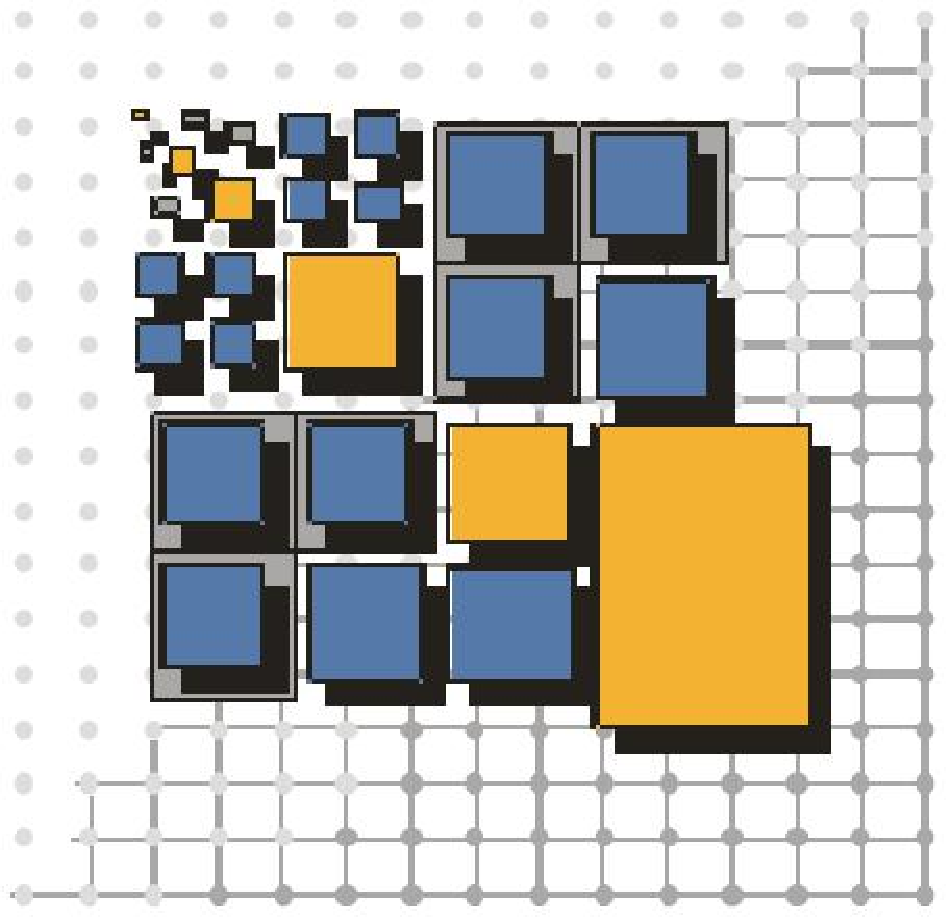
\includegraphics[height=26mm]{includes/vs-logo}
\end{minipage}
\hfill
\begin{minipage}{9cm}
  \centering
    Otto-Friedrich-Universit�t Bamberg\\[12pt]
    {\Large Lehrstuhl f�r Praktische Informatik}
\end{minipage}
\hfill
\begin{minipage}{3cm}
    
\includegraphics[height=26mm]{includes/UB-Logo-neu_blau-cmyk}
\end{minipage}
\end{minipage}\\[130pt]
{\LARGE #1}\\[24pt]
im Studiengang #2\\
der Fakult�t Wirtschaftsinformatik und Angewandte Informatik\\
der Otto-Friedrich-Universit�t Bamberg\\[90pt]
Zum Thema:\\[24pt]
{\Huge #3}\\[60pt]
\vfill
\begin{minipage}{\textwidth}
\center
Vorgelegt von:\\
{\Large #4\\[12pt]}
Themensteller:\\
Prof. Dr. Guido Wirtz\\[12pt]
Abgabedatum:\\
#5\\
\end{minipage}
\end{titlepage}
}
%
% Anweisung zur Erstellung der Eigenst�ndigkeitserkl�rung
% #1 = Typ der Arbeit
% #2 = Datum
% #3 = Vorname Name
\newcommand{\makedeclaration}[3]
{
	\fancyhead[LO]{\footnotesize\sc\nouppercase{Eigenst�ndigkeitserkl�rung}}
	%
			\vspace*{18cm}
			Ich erkl�re hiermit gem�� �17 Abs. 2 APO, dass ich die vorstehende #1 selbstst�ndig verfasst 
			und keine anderen als die angegebenen Quellen und Hilfsmittel benutzt habe.\\
			\vspace*{1cm}
			
			Bamberg, den #2 \hspace{5cm} #3
	%
}
%
% Wird f�r Hintergrund von Codelistings ben�tigt
\definecolor{hellgrau}{gray}{0.9}
%
% Einstellungen f�r Java-Code
\lstdefinestyle{javaStyle}{%
  basicstyle=\small,%
  backgroundcolor=\color{hellgrau},%
  keywordstyle=\bfseries,%
  showstringspaces=false,%
  language=Java,%
  numbers=left,%
  numberstyle=\tiny,%
  stepnumber=1,%
  numbersep=5pt,%
  extendedchars=true,%
  xleftmargin=2em,%
  lineskip=-1pt,%
  breaklines%
}
%
% neues environment f�r Java-Sourcecode
% #1 = "caption={Hier eigene �berschrift}, label={Hier eigenes Label}"
\lstnewenvironment{javacode}[1][]{%
\lstset{style=javaStyle,#1}%
}{}
%
% Befehl zum Einbinden von Java-Sourcecode aus Datei
% #1 = Dateiname relativ zu src-Verzeichnis
% #2 = �berschrift
% #3 = Label
\newcommand{\javafile}[3]{%
   \lstinputlisting[%
     caption={#2},%
     label={#3},%
     style=javaStyle]{src/#1}%
}
%
% Einbindung eines Bildes
% #1 = label f�r \ref-Verweise
% #2 = Name des Bildes ohne Endung relativ zu images-Verzeichnis
% #3 = Beschriftung
% #4 = Breite des Bildes im Dokument in cm
\newcommand{\bild}[4]{%
  \begin{figure}[htb]%
    \begin{center}%
      \includegraphics[width=#4cm]{images/#2}%
      \vskip -0.3cm%
      \caption{#3}%
      \vskip -0,2cm%
      \label{#1}%
    \end{center}%
  \end{figure}%
}
%
% Umgebung f�r Fliesstext um Grafik
% #1 = Ausrichtung: r, l, i, ...
% #2 = Breite des Bildes in cm
% #3 = Name des Bildes ohne Endung relativ zu images-Verzeichnis
% #4 = Beschriftung
% #5 = label f�r \ref-Verweise
\newcommand{\fliesstext}[5]{%
\begin{wrapfigure}{#1}{#2cm}%
\includegraphics[width=#2cm]{images/#3}%
\caption{#4}%
\label{#5}%
\end{wrapfigure}%
}
%%% Local Variables:
%%% mode: latex
%%% TeX-master: t
%%% End:


\begin{document}

% Titelblatt erstellen
\maketitle{Bachelor}{Wirtschaftsinformatik}{Automatisierung der Datenerfassung f�r Wissensdatenbanken im technischen Kontext}{Vasilyev Petr}{31.03.2017}

% Erstellung der Inhaltsverzeichnisses
\pagenumbering{Roman}

\tableofcontents
\newpage

\listoffigures
\newpage

%\listoftablesD
%\newpage

%\lstlistoflistings
%\newpage

\fancyhead[LO]{\footnotesize\sc\nouppercase{Abk�rzungsverzeichnis}}
\section*{Abk�rzungsverzeichnis}
% In Klammern steht das l�ngste Akronym!
\begin{acronym}[MVVM]
 \acro{API}{Application Programming Interface}
 \acro{DOM}{Document Object Model}
 \acro{DSS}{Decision Support System}
 \acro{DTD}{Document Type Definition}
 \acro{HTML}{Hypertext Markup Language}
 \acro{HTTP}{Hypertext Transfer Protocol}
 \acro{JSON}{JavaScript Object Notation}
 \acro{MVVM}{Model View ViewModel}
 \acro{PaaS}{Platform-as-a-Service}
 \acro{REST}{Representational State Transfer}
 \acro{SHA}{Secure Hash Algorithm}
 \acro{URI}{Uniform Resource Identifier}
 \acro{URL}{Uniform Resource Locator}
 \acro{XML}{Extensible Markup Language}
 \acro{XPath}{XML Path Language}
\end{acronym}
\newpage
\fancyhead[LO]{\footnotesize\sc\nouppercase{\leftmark}}
\setcounter{page}{1}
\pagenumbering{arabic}

%
% Einzelne Kapitel mit \input{sections/Kapitel-File} einf�gen.
%
\section{Einf�hrung}\label{sec:Einf�hrung}
\subsection{Motivation}\label{subsec:Motivation}
Die Idee von wissensbasierten Systemen entstand aus dem Anliegen, ein intelligentes System zu schaffen, das mithilfe des spezifischen Wissens die Menschen bei den Probleml�sungen unterst�tzt \cite[S.18]{akerkar2010}. Darin besteht der Unterschied zwischen einem konventionellen Informationssystem und einem wissensbasierten System. Informationssysteme sind schlie�lich datenbasiert und konzentrieren sich auf die Datenverarbeitung \cite[S.19]{akerkar2010}. Eine Spezialisierung der wissensbasierten Systeme stellen Expertensysteme dar, in denen das Wissen letztendlich von Experten stammt. Ein wissensbasiertes System bzw. ein Expertensystem ist durch die Trennung zwischen der Wissensdarstellung eines Problembereichs und der Wissensverarbeitung gekennzeichnet \cite[S.11]{beierle2014}.\\ 
Die Beschreibung des Wissens von einem wissensbasierten bzw. Expertensystem erfolgt in der Wissensbasis, die in Form einer Wissensdatenbank realisiert wird. Die initiale Datenbank wird in der Regel mithilfe manueller Datenerfassung aufgebaut \cite[S.70]{kurbel1992}. Ein Interview zwischen einem Wissensingenieurs und einem Wissenstr�ger wird beispielsweise oft eingesetzt \cite[S.76]{gottlob1990}. Allerdings sind die manuellen Wissenserwerbsmethoden f�r die Weiterentwicklung der Wissensbasis hinsichtlich der Erweiterung und Aktualisierung der Wissensdatenbank eher schlecht geeignet, da sie fehleranf�llig, kosten- und zeitintensiv sind. Aus diesem Grund wird seit langem versucht, den Prozess der Datenerfassung zu automatisieren. Eine Auswahl an bestehenden Ans�tzen, die bez�glich der vorliegenden Arbeit relevant sind, wird im Abschnitt zu den verwandten Arbeiten gegeben. Trotz der vielen Herangehensweisen gibt es kein einheitliches Konzept, das einen allgemeinen Rahmen f�r die Automatisierung der Datenerfassung bildet.
\subsection{Verwandte Arbeiten}\label{subsec:Verwandte-Arbeiten}
Ein Konzept der Automatisierung der Wissenserfassung wird in \cite{gebus2009} vorgestellt. Die Entwicklung der Wissensbasis umfasst dabei drei Phasen. In der ersten Phase wird die initiale Wissensdatenbank aufgebaut, die unvollst�ndig und teilweise widerspr�chlich sein kann. Die zweite Phase umfasst inkrementelle Erweiterung und Verbesserung der Wissensbasis. Dabei werden Methoden des maschinellen Lernens eingesetzt. Im Laufe der dritten Phase wird die Wissensbasis in Bezug auf Effizienz optimiert \cite[S.1444]{tecuci1992}. Gheorghe Tecuci betont, dass bei jeder Phase eine Kooperation zwischen dem fachlichen Experten und dem System notwendig ist. Nach der maschinellen Datenerschlie�ung werden die Ergebnisse manuell kontrolliert und anschlie�end in der Wissensbasis gespeichert. In dieser Weise lassen sich die Vorteile maschineller und manueller Datenerfassung optimal kombinieren \cite[S.137]{tecuci1994}, \cite[S.1445]{tecuci1992}.\\
Ein weiterer Ansatz wird in \cite{gebus2009} thematisiert. Dabei handelt es sich um ein datenbasiertes \acf{DSS}, das die Unternehmensf�hrung bei den Entscheidungen in Bezug auf die Produktionsoptimierung unterst�tzen soll. Allerdings werden die St�rungen in der Produktion von Anlagenbedienern (Experten) mittels Erfahrungswissen intern behoben, ohne dieses Wissen weiterzugeben. Als Folge hat die Unternehmensf�hrung kein umfangreiches Bild der Produktion und kann keine optimalen Entscheidungen treffen. Aus diesem Grund erweitern Gebus und Leivisk{\"a} das bestehende DSS mit einer Schnittstelle, um das Expertenwissen in die Datenbank zu integrieren \cite[S.94]{gebus2009}. Allgemeiner betrachtet geht es um die Transformation eines datenbasiertes System in ein wissensbasiertes System. Auch hier wird versucht, die Daten mithilfe der engen Kooperation zwischen dem Menschen und dem System zu erfassen. 
\subsection{Zielsetzung}\label{subsec:Zielsetzung}
Das Ziel der vorliegenden Arbeit ist die Erarbeitung eines allgemeinen Konzeptes zur Automatisierung der Datenerfassung. Da die komplett automatisierte Datenerfassung sehr schwierig umzusetzen ist, liegt der Schwerpunkt dieser Arbeit auf der Kombination zwischen den manuellen und maschinellen Vorgehensweisen.\\
Beim technischen Kontext wird angedeutet, dass die Umsetzung im Rahmen eines bestimmten Anwendungsbereichs erfolgt. Es wird also kein Allgemeinwissen wie in \cite{tandon2016}, sondern ein anwendungsbezogenes Wissen betrachtet. In diesem Zusammenhang wird das Konzept auf Basis eines Expertensystems entwickelt, da die Wissensbasis eines Expertensystems spezifischer ist als bei einem wissensbasierten System.\\
Die praktische Umsetzung soll auf Basis von \textit{PaaSfinder}\footnote{https://paasfinder.org} erfolgen. Bei \textit{PaaSfinder} handelt es sich um eine Web-Anwendung, die �ber eine Wissensdatenbank im Bereich \ac{PaaS} verf�gt. \ac{PaaS} geh�rt neben \ac{IaaS} und \ac{SaaS} zum Themengebiet von Cloud Computing \cite{nist2011} und soll die Anwendungsentwicklung erleichtern, indem die Laufzeit- ober Entwicklungsumgebungen von einem \ac{PaaS}-Anbieter dem Kunden vorkonfiguriert angeboten werden \cite[S.14]{lawton2008}. Da \textit{PaaSfinder} ein Open-Source Projekt ist, kann jeder der Datenbank von \textit{PaaSfinder} beitragen. Allerdings ist die Mitwirkung mit einem hohen Aufwand verbunden und setzt Informatikkenntnisse voraus. Au�erdem werden die Daten von \textit{PaaSfinder} haupts�chlich auf den Webseiten von \ac{PaaS}-Anbietern manuell erfasst. Dies stellt ein hohes Entwicklungspotential, die Erfassung von solchen Daten zu automatisieren.
\subsection{Aufbau der Arbeit}\label{subsec:Aufbau-der-Arbeit}
Die vorliegende Arbeit ist wie folgt aufgebaut. In Kapitel 2 wird der Begriff und die grundlegende Architektur eines Expertensystems erl�utert. Darauffolgend werden die Bestandteile, die f�r das Konzept relevant sind, n�her betrachtet. Anschlie�end wird schematisch das Kontext der Datenerfassung dargestellt und Automatisierungsm�glichkeiten angesprochen. In Kapitel 3 wird genauer auf die Automatisierungsmethoden bei der Datenerfassung eingegangen. Dabei werden bestehende Forschungsergebnisse vorgestellt und konzeptuell verallgemeinert. Kapitel 4 umfasst die praktische Umsetzung der Erkenntnisse, in Kapitel 2 und 3 gewonnen wurden. In Kapitel 5 wird die Implementierung evaluiert und die Ergebnisse der Arbeit zusammengefasst. Anschlie�end wird in Kapitel 7 ein Ausblick f�r zuk�nftige Forschung im betrachteten Bereich gegeben.
\newpage
\section{Grundlagen von Expertensystemen}\label{sec:Grundlagen}
\subsection{Begriffsdefinition}\label{subsec:Begriffsdefinition}
Urspr�nglich waren Expertensysteme Anwendungsprogramme, die logische Schlussfolgerungen aus einer Wissensbasis ziehen konnten. Au�erdem konnten sie �berpr�fen, ob eine Aussage aus einer vorhandenen Wissensbasis abgeleitet werden kann \cite[S.75]{greer2010}. Daher handelt es sich in der fr�heren Literatur meist um Anwendungen, die ihr Wissen in Form von logischen Ausdr�cken darstellen und in der Lage waren, neue Erkenntnisse vom bestehenden Wissen abzuleiten \cite{tecuci1992}. Im Laufe der Zeit hat sich das Konzept eines Expertensystems auf andere Anwendungsbereiche verbreitet. Aus diesem Grund gibt es mehrere Definitionen, die im Allgemeinen �hnlich sind und im Spezifischen Merkmale des zugeh�rigen Anwendungsbereichs beinhalten.\\
Allgemein l�sst sich sagen, dass ein Expertensystem ein Computersystem (Hardware und Software) ist, das in einem bestimmten Bereich Wissen und Schlussfolgerungsf�higkeit eines menschlichen Experten nachbildet \cite[S.12]{beierle2014}. Aus Sicht der Wirtschaftsinformatik zielen Expertensysteme drauf ab, das Expertenwissen menschlicher Fachleute in der Wissensbasis eines Computers abzuspeichern und f�r eine Vielzahl von Probleml�sungen zu nutzen \cite[S.59]{mertens2012}. Im Weiteren gehen Beierle und Kern-Isberner auf die Eigenschaften ein, die ein Expertensystem aufweisen soll \cite[S.12]{beierle2014}. Im Rahmen dieser Arbeit sind folgende Eingenschaften besonders relevant:
\begin{itemize}
\item Anwendung des Wissens eines oder mehrerer Experten, um Probleme in einem bestimmten Anwendungsbereich zu l�sen.
\item Leicht lesbare Wissensdarstellung.
\item M�glichst anschauliche und intuitive Benutzerschnittstelle.
\item Leichte Wartbarkeit und Erweiterbarkeit des Wissens im Expertensystem.
\item Unterst�tzung beim Wissenstransfer vom Experten zum System.
\end{itemize}
Es ist auch wichtig anzumerken, dass die Begriffe \grqq{}K�nstliche Intelligenz\grqq{}, \grqq{}Wissensbasiertes System\grqq{} und \grqq{}Expertensystem\grqq{} in einer engen Beziehung zueinander stehen. Haun gibt eine systematische Abgrenzung dieser Begriffe, die sich folgenderma�en beschreiben l�sst \cite[S.30]{haun2000}:
\begin{itemize}
\item \textit{K�nstliche Intelligenz} stellt den Oberbegriff dar und bildet den theoretischen Rahmen f�r die Entwicklung von Wissensbasierten Systemen und Expertensystemen.
\item \textit{Wissensbasierte Systeme} sind eine Teilmenge der Anwendungen der k�nstlichen Intelligenz. Sie wenden die Wissensverarbeitung auf ein konkretes Aufgabengebiet an und verwalten Allgemeinwissen explizit und getrennt vom Rest des Systems.
\item \textit{Expertensysteme}, die ein Teilbereich der Wissensbasierten Systeme sind, stellen eine Spezialisierung von Wissensbasierten Systemen dar. Sie verwalten spezifisches Expertenwissen, das von einem Experten stammt und auf praxisbezogene Probleme angewandt wird.
\end{itemize}
Graphisch l�sst sich die vorliegende Abgrenzung in der Abbildung \ref{Abgrenzung} darstellen:
\begin{figure}[H] 
	\centering
	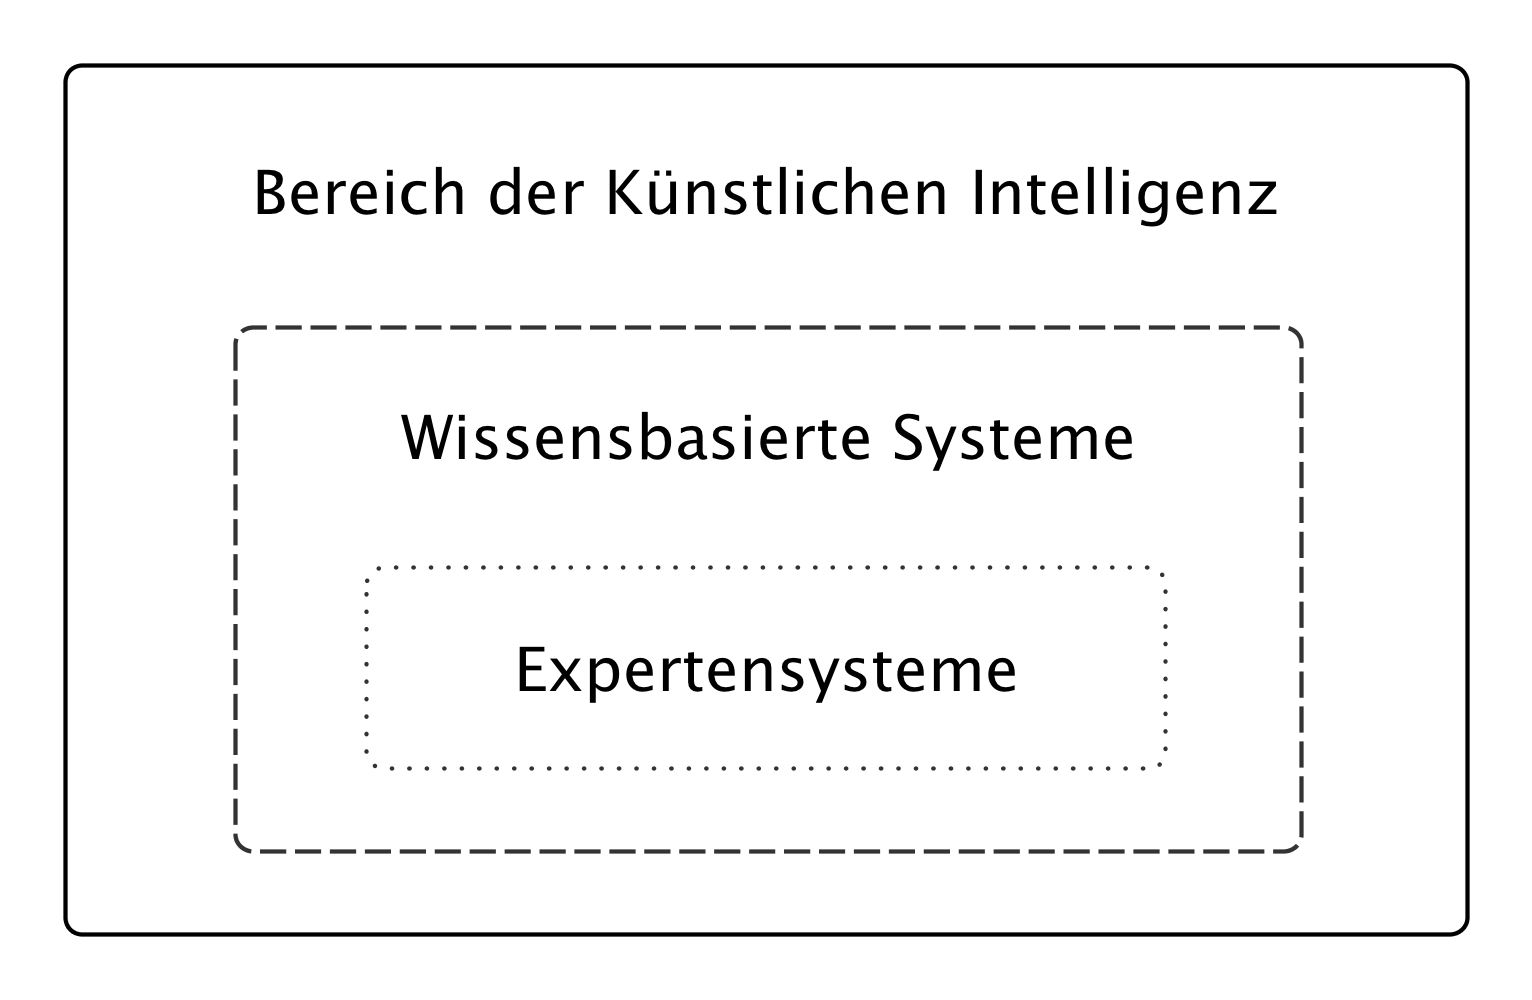
\includegraphics[width=0.55\textwidth]{images/abgrenzung.png}
	\caption{Begriffsabgrenzung, \cite[S.30]{haun2000}}
	\label{Abgrenzung}
\end{figure} 
Nach dieser Agbrenzung l�sst sich feststellen, dass der Unterschied zwischen einem Wissensbasierten System und einem Expertensystem darin besteht, dass das Wissen im Endeffekt von einem Experten stammt. Allerdings ist dieses Kriterium zu einfach und nicht besonders aussagekr�ftig. Beierle und Kern-Isberner weisen drauf hin, dass nach diesem Kriterium viele existierenden Wissensbasierten Systeme als Expertensysteme bezeichnet werden k�nnten \cite[S.11]{beierle2014}. Aufgrund dessen stellen die Autoren die Eigenschaften eines Experten dar, die sich folgenderma�en zusammenfassen lassen:
\begin{itemize}
\item Experten sind selten und teuer.
\item Experten sind nicht immer verf�gbar.
\item Leistungsf�higkeit der Experten ist nicht konstant, sondern kann nach Tagesverlauf schwanken.
\item Expertenwissen kann oft nicht als solches weitergegeben werden.
\item Expertenwissen kann verloren gehen.
\end{itemize}
Ein gutes Beispiel hinsichtlich der Gefahr, dass Expertenwissen verloren gehen kann, wird in \cite[S.94]{gebus2009} vorgestellt. Gebus nimmt den Bezug auf die Mitarbeiter der sogenannten Baby-Boomgeneration. Es handelt sich um Experten, die ein umfangreiches Erfahrungswissen besitzen und bald aus Altersgr�nden das Unternehmen verlassen. Somit geht auch das Erfahrungswissen aus dem Unternehmen verloren.\\
Zusammenfassend l�sst sich sagen, dass die Entwicklung eines Expertensystems eine hohes Potenzial besitzt. Allerdings kann ein Expertensystem nicht als Ersatz eines menschlichen Experten betrachtet werden. Vielmehr geht es um eine Erfassung, Darstellung und Pflege des Expertenwissens in einem Expertensystems, um die Arbeitsprozesse effizienter zu gestalten und sowohl erfahrene als auch neue Anwender in einem bestimmten Wissensbereich bei der Aufgabenabwicklung zu unterst�tzen.
\subsection{Architektur eines Expertensystems}\label{subsec:Architektur}
Beierle und Kern-Isberner betonen, dass die Trennung zwischen der Darstellung des Wissens (Wissensbasis) und der Wissensverarbeitung (Wissensverarbeitungskomponente) der wichtigste Aspekt eines Wissensbasierten Systems ist. \cite[S.11]{beierle2014}. Die Wissensbasis kann man sich als eine Art Datenstruktur vorstellen, in der das ben�tigte Wissen gespeichert wird. Die Wissensverarbeitungskomponente umfasst eine Menge von anwendungsunabh�ngigen Algorithmen, die mithilfe der Wissensbasis eine L�sung f�r ein gegebenes Problem erarbeiten. Somit stehen die Wissensbasis und die Wissensverarbeitungskomponente in einer engen Beziehung zueinander \cite[S.18]{kurbel1992}.\\
Allgemein umfasst ein Expertensystem folgende Bestandteile \cite[S.75]{greer2010}:
\begin{itemize}
\item \textit{Wissensbasis}, die Expertenwissen in Form von Fakten in einer bestimmten Sprache speichert sowie Regeln zur Wissensorganisation beinhaltet.
\item \textit{Inferenzmaschine}, die unter Ber�cksichtigung des zugrunde liegenden Wissensbedarfs die Wissensbasis
durchsucht bis das System einen Probleml�sungsvorschlag erarbeitet hat oder herausfindet, dass keiner existiert.
\item \textit{Dialogkomponente}, die eine Schnittstelle zwischen dem Nutzer und dem System darstellt. 
\item \textit{Erkl�rungskomponente}, die dem Benutzer erl�utert, warum und auf welche Weise eine bestimmte L�sung gefunden bzw. nicht gefunden wurde \cite[S.126]{haun2000}.
\item \textit{Wissensakquisitionskomponente}, die den Entwickler des Expertensystems bei der Erweiterung, �nderung und Wartung der Wissensbasis unterst�tzt.
\end{itemize}
Laut Tecuci stellen Wissensbasis und Inferenzmaschine grundlegende Bestandteile eines Expertensystems dar und bilden damit den Kern des Expertensystems \cite[S.1444]{tecuci1992}. Dialogkomponente, Erkl�rungskomponente und Wissensakquisitionskomponente geh�ren zur sogenannten Schale und sind f�r die Kommunikation zwischen dem Systemverwalter und dem Nutzer zust�ndig (siehe Abbildung \ref{expertensystem_haun}). 
\begin{figure}[H] 
	\centering
	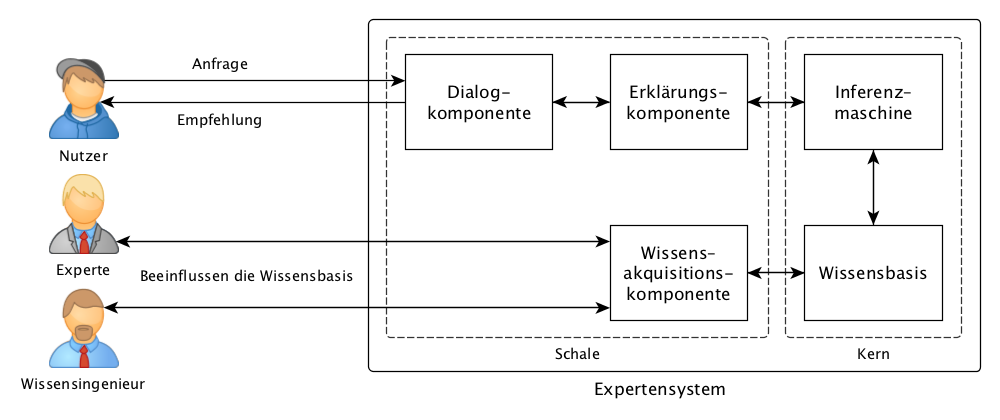
\includegraphics[width=1.0\textwidth]{images/expertensystem_haun.png}
	\caption{Architektur eines Expertensystems nach Haun, \cite[S.126]{haun2000}}
	\label{expertensystem_haun}
\end{figure}
Im Hinblick auf die Interaktion gibt es drei Gruppen, die mit dem Expertensystem interagieren: 
\begin{itemize}
\item \textit{Nutzer}, der das Expertensystem zum L�sen eines Problems benutzt und mit der Dialogkomponente kommuniziert. Der Wissensingenieur und der Experte k�nnen ebenso als Nutzer auftreten \cite[S.758]{wachsmuth1993}.
\item \textit{Wissensingenieur}, der sich mit dem Aufbau und Wartung der Wissensbasis besch�ftigt. Unter anderem ist Wissensmodellierung ein wichtiger Aufgabenbereich eines Wissensingenieurs \cite[S.742]{wachsmuth1993}.
\item \textit{Experte}, der �ber spezifisches Erfahrungswissen verf�gt, das f�r das Expertensystem relevant ist.
\end{itemize}
Der Ablauf der Kommunikation zwischen dem Nutzer und dem Expertensystem sieht folgenderma�en aus: 
\begin{itemize}
\item Der Nutzer schickt eine Anfrage an die Dialogkomponente des Expertensystems.
\item Die Dialogkomponente �bermittelt die Anfrage an die Inferenzmaschine.
\item Die Inferenzmaschine erarbeitet eine L�sung f�r das gegebene Problem mittels der Wissensbasis und gibt das Ergebnis an die Dialogkomponente zur�ck. 
\item Anschlie�end teilt die Dialogkomponente dem Nutzer die L�sung des Problems mit. Falls keine L�sung zum Problem existiert, wird eine entsprechende Fehlermeldung angezeigt.
\end{itemize}
Auf der anderen Seite k�nnen die Inhalte der Wissensbasis von einem Wissensingenieur mithilfe der Wissensakquisitionskomponente beeinflusst werden. Der Wissenserwerb durch den Wissensingenieur ist die verbreitetste Vorgehensweise, neue Daten f�r ein wissensbasiertes System zu erschlie�en. Meistens handelt es sich um ein Interview zwischen dem Wissensingenieur und dem Experten \cite[S.76]{greer2010}, \cite[S.210]{fujihara1997}. Neben dem Interview kann der Wissensingenieur eine Recherche der verf�gbaren Wissensquellen wie Text, technische Zeichnungen oder Web-Ressourcen durchf�hren. Anschlie�end werden die Daten vom Wissensingenieur formalisiert und in die Wissensbasis gespeichert. \\
Die Wissensbasis kann in einigen F�llen von einem fachlichen Experten beeinflusst werden. Daf�r ist eine geeignete Expertenschnittstelle innerhalb der Wissensakquisitionskomponente notwendig, die den Experten erm�glicht, ihr Erfahrungswissen selbst zu formalisieren und gegebenenfalls zu warten \cite[S.743]{wachsmuth1993}. Die �berpr�fung des Dateninputs ist ebenfalls die Aufgabe der Wissensakquisitionskomponente. Dies kann mittels Durchf�hrung automatisierten Tests bei jeder �nderungsanfrage erfolgen, um die Konsistenz der Wissensbasis zu gew�hrleisten \cite[S.743]{wachsmuth1993}.\\
Um ein geeignetes Konzept der automatisierten Datenerfassung zu entwickeln, ist ein grundlegendes Verst�ndnis von der Struktur und Funktionsweise der Wissensbasis sowie der Wissensakquisitionskomponente erforderlich. Im weiteren Verlauf der Arbeit werden die Erkenntnisse �ber die Wissensbasis und die Wissensakquisitionskomponente erl�utert, die in der Forschung von Expertensystemen entstanden sind.

\subsection{Wissensbasis}
Neben der Inferenzmaschine stellt die Wissensbasis den zentralen Teil eines Expertensystems, der die Daten des gesamten Systems beinhaltet \cite[S.754]{wachsmuth1993}. Im Folgenden werden der allgemeine Prozess der Wissensbasisentwicklung, der Inhalt der Wissensbasis und die M�glichkeiten der Wissensrepr�sentation thematisiert. Gheorghe Tecuci beschreibt folgende Phasen bei der Entwicklung der Wissensbasis \cite[S.1444]{tecuci1992}: 
\begin{itemize}
\item[1.] Systematische Erfassung vom Expertenwissen
\item[2.] Verfeinerung der Wissensbasis
\item[3.] Reorganisation der Wissensbasis
\end{itemize}
In der ersten Phase werden das Vokabular und die geeignete Wissensrepr�sentation festgelegt. Gebus und Leivisk{\"a} betonen, dass die Wissensrepr�sentation den entscheidenden Einfluss auf die Generierung und sp�tere Handhabung der Wissensbasis hat \cite[S.95]{gebus2009}. Die initialen Daten werden meistens im Rahmen eines Interviews zwischen dem Wissensingenieur und dem Experten erfasst \cite[S.1444]{tecuci1992}. Das Ergebnis der ersten Phase ist eine initiale Wissensbasis, die unvollst�ndig und teilweise widerspr�chlich ist. In der zweiten Phase wird die initiale Wissensbasis mithilfe der geeigneten Datenerfassungsmethoden solange erweitert und verbessert, bis sie vollst�ndig und korrekt genug ist, um ein gegebenes Problem richtig zu l�sen. In der dritten Phase wird die vollst�ndige und korrekte Wissensbasis reorganisiert, um die Effizienz der L�sungsberechnung zu steigern \cite[S.1445]{tecuci1992}. Zusammenfassend werden die Phasen in der Abbildung \ref{drei_phasen} dargestellt.  
\begin{figure}[H] 
	\centering
	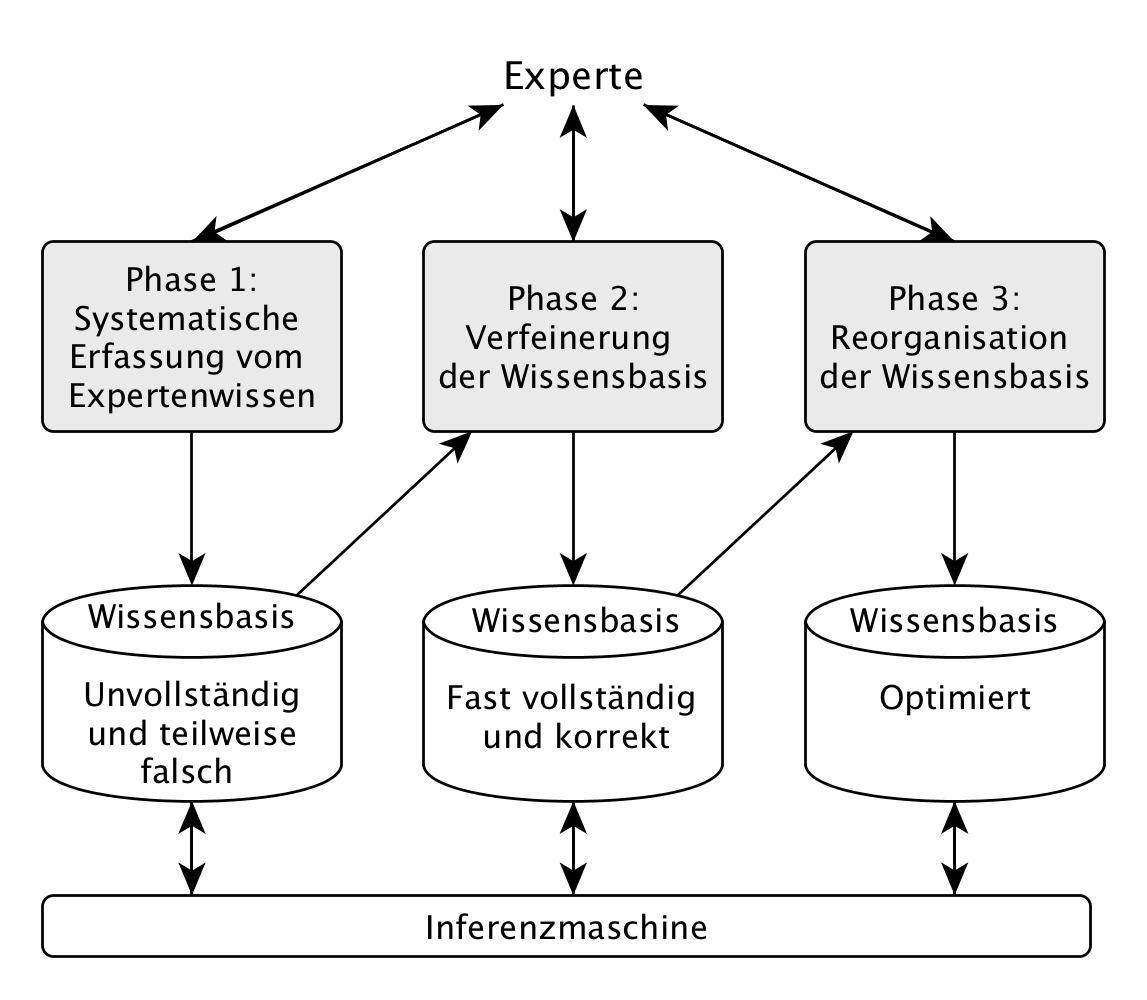
\includegraphics[width=0.7\textwidth]{images/drei_phasen.png}
	\caption{Phasen der Expertensystementwicklung, \cite[S.138]{tecuci1994}}
	\label{drei_phasen}
\end{figure}
In der Abbildung \ref{drei_phasen} sieht man, dass der Autor dem Experten die gesamte Kontrolle �ber die Entwicklung der Wissensbasis zuweist. Allerdings ist diese Sichtweise nicht vollst�ndig, da im Entwicklungsprozess der Wissensingenieur und der Systementwickler beteiligt sind und dementsprechend ber�cksichtigt werden sollen.\\
In Bezug auf den Inhalt der Wissensbasis unterscheiden Beierle und Kern-Isberner folgende Wissensarten \cite[S.5]{beierle2014}:
\begin{itemize}
\item \textit{Fachspezifisches Wissen}. Dabei handelt es sich um das spezifischste Wissen, das sich
nur auf den gerade betrachteten Problemfall bezieht. Das sind z.B. Fakten, die von Beobachtungen oder Untersuchungsergebnissen stammen.
\item \textit{Regelhaftes Wissen}, das den eigentlichen Kern der Wissensbasis darstellt. Dieses Wissen kann noch genauer differenziert werden: 
	\begin{itemize}
	\item \textit{Bereichsbezogenes Wissen}, das sich auf den gesamten Problembereich beziehen. Das kann sowohl theoretisches Fachwissen als auch Erfahrungswissen sein. Anders gesagt handelt es sich um generisches Wissen.
	\item \textit{Allgemeinwissen}, das z.B. um generelle Probleml�sungsheuristiken, Optimierungsregeln oder auch allgemeines Wissen �ber Objekte und Beziehungen in der realen Welt beinhaltet.
	\end{itemize}
\end{itemize}
Unter Ber�cksichtigung der Differenzierung der Wissensarten innerhalb der Wissensbasis beschreiben die Autoren in \cite[S.18]{beierle2014} auf eigene Weise die Architektur des Expertensystems, die in der Abbildung \ref{expertensystem_beierle}  dargestellt wird.
\begin{figure}[H] 
	\centering
	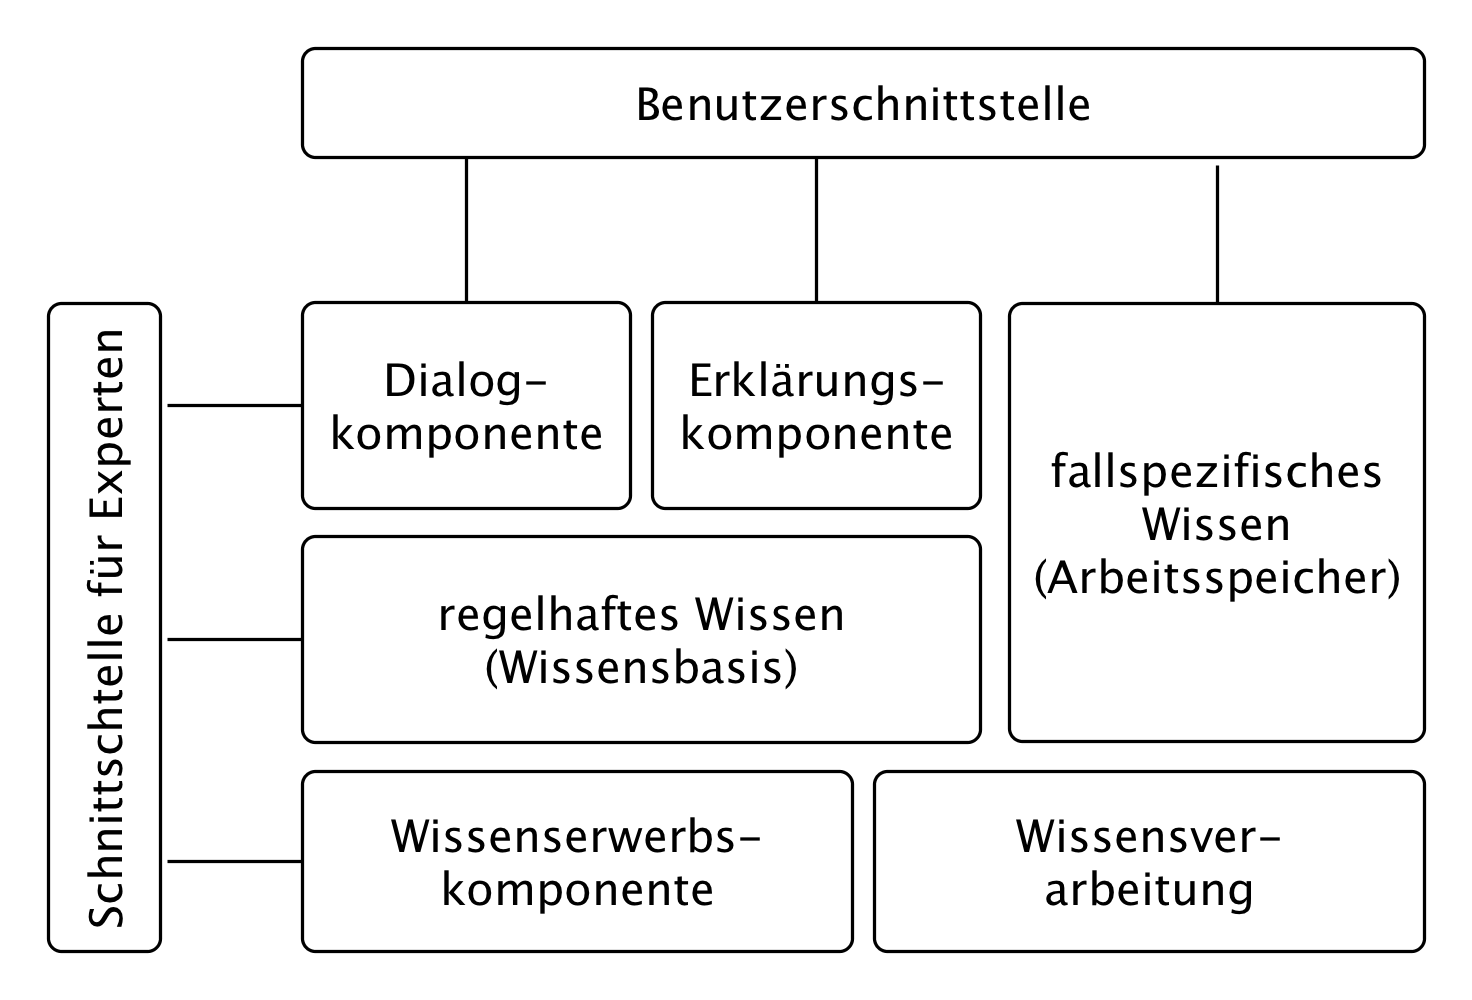
\includegraphics[width=0.7\textwidth]{images/expertensystem_beierle.png}
	\caption{Expertensystems nach Beierle und Kern-Isberner, \cite[S.18]{beierle2014}}
	\label{expertensystem_beierle}
\end{figure} 
Laut Beierle und Kern-Isberner k�nnen verschiedene Wissensarten in einem wissensbasierten System je nach dem Anwendunsgbereich unterschiedli umfangreich auftreten. Ein hochspezialisiertes System kann beispielsweise �ber sehr wenig oder gar kein Allgemeinwissen verf�gen. Auf der anderen Seite kann ein wissensbasiertes System den Schwerpunkt auf das gew�hnliche Alltagswissen legen \cite[S.5-6]{beierle2014}.\\
Ein weiterer Aspekt beim Aufbau der Wissensbasis ist die Wissensrepr�sentation. Die grundlegende Aufgabe der Wissensrepr�sentation ist die Formularisierung von Wissen, um eine maschinelle Verarbeitung  erst zu erm�glichen \cite[S.22]{haun2000}. Sinz und Ferstl unterscheiden folgende Formen der Wissensrepr�sentation \cite[S.366]{sinz2013}:
\begin{itemize}
\item \textit{Regelorientierte Darstellung}, in der das Wissen als (WENN, DANN)-Beziehungen beschrieben wird. Diese Darstellungsform wird beispielsweise bei Prolog-Regeln eingesetzt.
\item \textit{Objektorientierte Darstellung}, die das Konzept der Objekttypen �bernimmt und mit deklarativen Operatorbeschreibungen verbindet.
\item \textit{Constraints Darstellung}, die Modellbeschreibungen aus dem Operations Research benutzt. Dabei handelt es sich um L�sungsr�ume durch Nebenbedingungen und Zielvorgaben.   
\end{itemize}
Hinsichtlich der Wissensrepr�sentation stellen Ferstl und Sinz imperative und deklarative Paradigmen gegen�ber \cite[S.366]{sinz2013}. Ein Programm, das dem imperativen Paradigma folgt, besteht aus einer Folge von Befehlen, die nacheinander ausgef�hrt werden \cite[S.341]{sinz2013}. Bei einem deklarativen Programm handelt es sich um eine Beschreibung der Aufgabenau�ensicht. Ein deklaratives Programm hat keine festgelegten L�sungsverfahren je Aufgaben. Stattdessen wird eine L�sung zum Zeitpunkt der Aufgabendurchf�hrung mittels Inferenzmaschine abgeleitet \cite[S.361]{sinz2013}.\\
Allgemein beziehen sich die Autoren darauf, dass an ein wissensbasiertes System nur geringe Anforderungen bez�glich Vollst�ndigkeit, Widerspruchsfreiheit und Eindeutigkeit gestellt werden k�nnen. Aus diesem Grund ist das deklarative Paradigma f�r die Wissensrepr�sentation besser geeignet. Folgende Gr�nde nennen die Autoren f�r die deklarative Umsetzung der Wissensbasis \cite[S.366]{sinz2013}: 
\begin{itemize}
\item \textit{Wissensdarstellung}: Da ein Mensch das Erfahrungswissen durch assoziative Beziehungsmuster aufbaut, ist die deklarative Wissensdarstellung eher geeignet.
\item \textit{Wissensauswertung}: �nderungen von Erfahrungswissen werden normalerweise in deklarativen Form erfasst.
\item \textit{Wissensverf�gbarkeit}: Die Codewartung von einem imperativen Programm ist fehleranf�llig, kosten- und zeitintensiv, da das Erfahrungswissen h�ufig ge�ndert und aktualisiert werden muss.
\end{itemize}
Der objektorientierte Ansatz ist eine weitere M�glichkeit, das Wissen zu beschreiben. Ein Beispiel f�r die objektorientierte Implementierung wird in \cite{leung1990} vorgestellt. Die Wissensbasis wird dabei als eine Sammlung von Klassen, Objekten und Methoden definiert \cite[S.40]{leung1990}. Der gro�e Vorteil solcher Umsetzung besteht in der Modularit�t des Wissens. Das Wissen in unabh�ngige Module aufgeteilt wird. Da die einzelnen Module unabh�ngig voneinander sind, k�nnen sie getrennt getestet und modifiziert werden, ohne den Rest der Wissensbasis zu beeintr�chtigen. Dies erm�glicht hohe Flexibilit�t bei der Wissensbasiserweiterung \cite[S.43]{leung1990}.\\
Neben der Implementierung der Wissensbasis ist eine geeignete Umsetzung der Wissensakquisitionskomponente erforderlich, um die Wissensbasis aktuell, m�glichst fehlerfrei und konsistent zu halten. Im Folgenden wird die Wissensakquisitionskomponente in Hinsicht auf den allgemeinen Aufbau und Funktionen thematisiert.  
\subsection{Wissenserwerbskomponente}\label{subsec:Wissenserwerbskomponente}
Bei der Wissenserwerbskomponente handelt es sich um einen Bestandteil eines Expertensystems, der den Wissensingenieur oder einen Experten beim Aufbau und sp�terer Erweiterung der Wissensbasis unterst�tzt \cite[S.18]{gottlob1990}. Allgemein umfasst die Wissenserwerbskomponente zwei grunds�tzliche Aufgaben, n�mlich den Wissenserwerb und die Pr�fung des Dateninputs auf Konsistenz, Vollst�ndigkeit und Einschr�nkungen des Expertensystems \cite[S.759]{wachsmuth1993}.\\
Unter dem Wissenserwerb wird eine �bertragung sowie Eingliederung von Wissen �ber Probleml�sungsverfahren in ein Computerprogramm verstanden \cite[S.178]{gottlob1990}. Es werden folgende Grundarten des Wissenserwerbs unterschieden \cite[S.742]{wachsmuth1993}:
\begin{itemize}
\item \textit{Indirekter Wissenserwerb}: Ein Wissensingenieur f�hrt ein Interview mit einem Experten, oder allgemein mit einem Wissenstr�ger. Die Analyse der Dokumente, die f�r das System relevant sind, geh�rt ebenso zur Aufgabe des Wissensingenieurs.
\item \textit{Direkter Wissenserwerb}: Ein Wissenstr�ger gibt sein Wissen selbst mittels einer Schnittstelle ins Expertensystem ein. 
\item \textit{Automatisierter Wissenserwerb:} Die Wissensbasis wird entweder mithilfe der automatisierten Datenerschlie�ung aus verf�gbarer Dokumente oder Methoden des maschinellen Lernens erweitert.
\end{itemize}
Die Methoden des indirekten Wissenserwerbs lassen sich grunds�tzlich in unstrukturierte und strukturierte Verfahren unterteilen. Das unstrukturierte Interview ist die am h�ufigsten verwendete Methode \cite[S.76]{gottlob1990}. Dabei stellt der Wissensingenieur dem Experten problembezogene Zwischenfragen, um ein m�glichst vollst�ndiges Bild des zur Probleml�sung erforderlichen Wissens zu bekommen. Die Hauptschwierigkeit bei der Wissenserhebung durch ein Interview ist die Formulierung der Fragen. Wenn die Fragen zu spezifisch sind, k�nnen wichtige Informationen ausgelassen werden \cite[S.95]{gebus2009}. Eine strukturierte Vorgehensweise der Wissenserhebung ist die Protokollanalyse, wobei der Experte beim L�sen eines Problems aufgezeichnet wird. Um den L�sungsweg nachvollziehbar zu machen, kann der Experte die Aufgabe gezielt langsamer durchf�hren oder die Aufzeichnung mit Kommentaren versehen. Die aufgabenbezogenen L�sungen werden mithilfe der Induktion generalisiert. Bei der Induktion wird eine allgemeine Regel aus den Einzelf�llen abgeleitet \cite[S.308]{castro2001}. Anschlie�end werden die erzielten Ergebnisse vom Wissensingenieur formalisiert und ins Expertensystem eingetragen.\\
Beim direkten Wissenserwerb soll eine geeignete Schnittstelle im Rahmen der Wissenserwerbskomponente zur Verf�gung gestellt werden, die es dem Wissenstr�ger erm�glicht, sein Wissen ins System einzugeben. Die Schnittstelle soll eine dem Wissenstr�ger bekannte Wissensrepr�sentation verwenden und benutzerfreundlich bei der Dateneingabe sein \cite[S.743]{wachsmuth1993}. Ein Beispiel der Benutzerfreundlichkeit ist gleichzeitige Validierung der Benutzereingaben sowie eine R�ckmeldung bei unzul�ssigen Aktionen. Der direkte Wissenserwerb hat den Vorteil, dass die Wissensbasis ohne den Wissensingenieur erweitert werden kann. Allerdings betonen die Autoren in \cite[S.765]{wachsmuth1993}, dass das nur in gut verstandenen und strukturierten Anwendungsbereichen m�glich sei.\\
Zu dem automatisierten Wissenserwerb gibt es am wenigsten Erkenntnisse, die allgemein anwendbar sind. Meistens handelt es sich um L�sungen, die nur innerhalb eines spezifischen Anwendungsbereichs funktionieren. Nichtsdestotrotz l�sst sich sagen, dass das Wissen sich entweder aus vorhandenen Daten (maschinelles Lernen) oder aus verf�gbaren Dokumenten (automatisierte Dokumentenanalyse) generieren l�sst \cite[S.78]{gottlob1990}. Die Implementierung h�ngt jedoch vom Anwendungsgebiet ab. Ein Beispiel f�r den Fall gro�er Datenmenge und Anwendung des maschinellen Lernens ist ein Diagnosesystem, das f�r m�gliche Diagnose F�lle mit Symptomen enth�lt. F�r die Textanalyse k�nnen beispielsweise Bedienungsanleitungen analysiert werden, wobei diese Vorgehensweise gewisse Einschr�nkungen ausweist. Die Schwierigkeit dabei besteht darin, dass das Erfahrungswissen nicht in den Textdokumenten zu finden ist \cite[S.79]{gottlob1990}.\\
In allen F�llen des Wissenserwerbs werden die Daten an die zentrale Schnittstelle weitergereicht. Diese Schnittstelle besch�ftigt sich mit der Zwischenspeicherung und der Pr�fung der Datens�tze auf Korrektheit, bevor die Daten endg�ltig in der Wissensbasis gespeichert werden. Zum Teil kann der Wertebereich direkt im einzelnen Modul des Wissenserwerbs eingeschr�nkt werden. Beispielsweise kann ein Eingabefeld in der Wissenstr�gerschnittstelle nur positive Zahlen zulassen. F�r den restlichen Teil werden automatisierte Tests durchgef�hrt, die sicherstellen, dass neue Daten keine Inkonsistenzen in Bezug auf die Einschr�nkungen der Wissensbasis erzeugen \cite[S.765]{wachsmuth1993}.\\
Zusammenfassend l�sst sich die Wissenserwerbskomponente schematisch in Abbildung \ref{wissenserwerbskomponente} wie folgt darstellen:
\begin{figure}[H] 
	\centering
	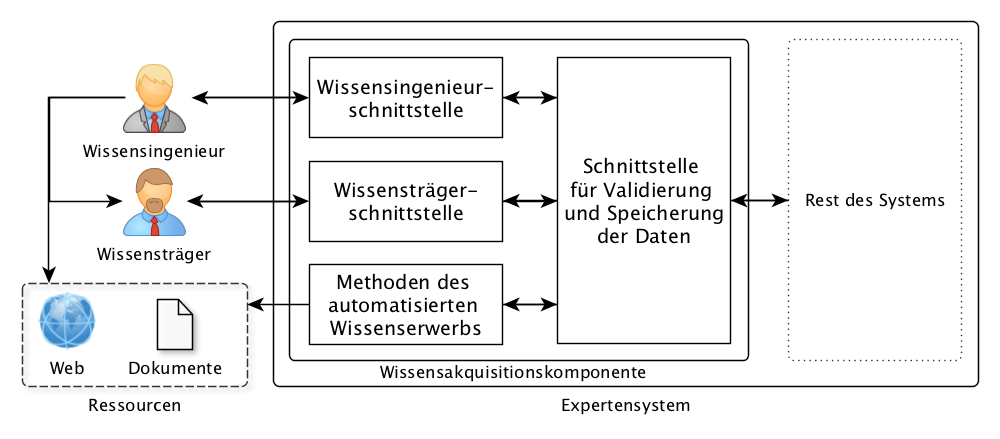
\includegraphics[width=1.0\textwidth]{images/wissenserwerbskomponente.png}
	\caption{Wissenserwerbskomponente}
	\label{wissenserwerbskomponente}
\end{figure}
In Abbildung \ref{wissenserwerbskomponente} sieht man deutlich, dass die Wissenserwerbskomponente modular aufgebaut ist. Allgemein kann dieses Modell in jedem Expertensystem eingesetzt werden, wobei die konkrete Umsetzung in Bezug auf den Anwendungsbereich spezifiziert wird. Dabei l�sst sich der Automatisierungsgrad der Datenerfassung leicht anpassen, indem der Schwerpunkt auf gew�nschte Bestandteile der Wissenserwerbskomponente gelegt wird. Beispielsweise kann sich ein Expertensystem mit umfangreichen Falldaten auf das maschinelle Lernen konzentrieren. Ein System, dass auf der Datenerfassung mithilfe der Wissenstr�gerschnittstelle basiert ist, wird in \cite[S.97]{gebus2009} vorgestellt.\\
Im weiteren Verlauf der Arbeit werden die Wissenstr�gerschnittstelle, die Komponente mit Methoden des automatisierten Wissenserwerbs und die Schnittstelle f�r Validierung und Speicherung der Daten thematisiert, da sie ein Potenzial f�r die Automatisierung der Datenerfassung aufweisen.
\newpage
\section{Automatisierung der Wissenserfassung}\label{sec:Datenerfassung}
Mit der Wissensakquisitionskomponente wurde bereits angedeutet, dass die Datenerfassung f�r Expertensysteme meistens nur teilweise automatisierbar ist. Die Autoren in \cite{tecuci1994} weisen ebenso darauf hin, dass manuelle und maschinelle Wissenserschlie�ung jeweils eigene St�rke haben, die gegenseitig nicht ersetzt werden k�nnen \cite[S.137]{tecuci1994}. Aus diesem Grund ist bei der Datenerfassung ein hybrides Modell sinnvoll, das die Vorteile manueller und maschineller Verfahren kombiniert. Aufgrund der Fragestellung dieser Arbeit wird es im weiteren auf automatisierte und halb-automatisiere Bestandteile der Wissensakquisitionskomponente beschr�nkt.
\subsection{Schnittstelle zur Dateneingabe}
Die Schnittstelle zur Dateneingabe (auch als Wissenstr�gerschnittstelle im Kapitel \ref{subsec:Wissenserwerbskomponente} bekannt) ist in der Regel ein Bestandteil eines Tools zum Wissenserwerb. Diese Schnittstelle soll dem Wissenstr�ger erm�glichen, sein Wissen ins System auf eine einfache Weise einzutragen. Da die Daten manuell eingegeben und maschinell verarbeitet werden, wird dieser Ansatz als semi-automatisiert bezeichnet. Im Zusammengang mit der Wissenstr�gerschnittstelle wurden zahlreiche Tools entwickelt (z.B. in \cite{rafea2003} oder \cite{gebus2009}), die sich in Automatisierungsgrad, Problembereich oder Benutzergruppe unterscheiden \cite[S.49]{rafea2003}. Im Folgenden wird eine Arbeit genauer betrachtet, die den Einsatz der Wissenstr�gerschnittstelle beispielhaft darstellt.\\
Das Praxisbeispiel wird in der \cite{gebus2009} vorgestellt und bezieht sich auf die Wissenserfassung aus der Produktion eines Elektrotechnikunternehmens. In der Fallstudie wird ein bereits bestehendes \acf{DSS} betrachtet, das die F�hrungskr�fte bei den Entscheidungen von nicht-strukturieren Problemen in der Produktion unterst�tzt \cite[S.94]{gebus2009}. Das DSS verf�gt bereits �ber eine Datenbank, die allerdings nur Daten von Produkteigenschaften enth�lt. Die eigentlichen Prozesse werden allerdings von Experten gesteuert, die mithilfe des Erfahrungswissens St�rungen in der Produktion beseitigen. Dieses Erfahrungswissen �ber St�rungen wird im System nicht erfasst. Als Folge hat die Unternehmensf�hrung einen begrenzten �berblick �ber die Situation in der Produktionsabteilung. Au�erdem besteht die Gefahr, dass das spezifische Expertenwissen verloren geht, falls der Wissenstr�ger das Unternehmen verl�sst \cite[S.467]{song2016}.\\
Die Zielsetzung von \cite{gebus2009} ist die Erfassung des Expertenwissens aus der Produktion und die Integration dieses Wissens in die Entscheidungsprozesse auf der Organisationsebene. Um das Wissen aus der Produktionsabteilung zu erschlie�en, erweitern Gebus und Leivisk{\"a} das bestehende System um eine Schnittstelle f�r Anlagenbediener. Die Umsetzung erfolgt in Form von einem Prototyp. Der Entwicklungsprozess l�sst sich allgemein wie folgt beschreiben:
\begin{itemize}
\item[1.] Die Definition der Zielgruppe, die f�r die Schnittstelle relevant ist.
\item[2.] Ausgehen von der Zielgruppe werden die Wissensrepr�sentation sowie funktionale und nicht-funktionale Anforderungen spezifiziert.
\item[3.] Die Umsetzung und Evaluation des Prototyps.
\end{itemize}
Im ersten Schritt definieren Gebus und Leivisk{\"a} die bestehenden Nutzergruppen des gesamten Systems \cite[S.97]{gebus2009}:
\begin{itemize}
\item Anlagenbediener (Experte), der sein Wissen zu den St�rungen mittels der Wissenstr�gerschnittstelle in die Datenbank eingibt.
\item Administrator, der das gesamte System verwaltet.
\item Qualit�tsabteilung, die die St�rungsstatistik analysiert, eine Qualit�tsr�ckmeldung an die Produktion und einen Bericht an die F�hrungskraft �bermittelt.
\item F�hrungskraft, die eine umfangreiche �bersicht von der Qualit�tsabteilung erh�lt und davon ausgehend Entscheidungen zur Prozessoptimierung trifft.
\end{itemize}
Im Rahmen der Fallstudie ist die Nutzergruppe der Anlagenbediener relevant, wobei das System jeder Nutzergruppe eine geeignete Benutzerschnittstelle zur Verf�gung stellt. Schematisch l�sst sich die Struktur und die Informationsfl�sse im DSS in der Abbildung \ref{dss_gebus} vereinfacht nachbilden.
\begin{figure}[H] 
	\centering
	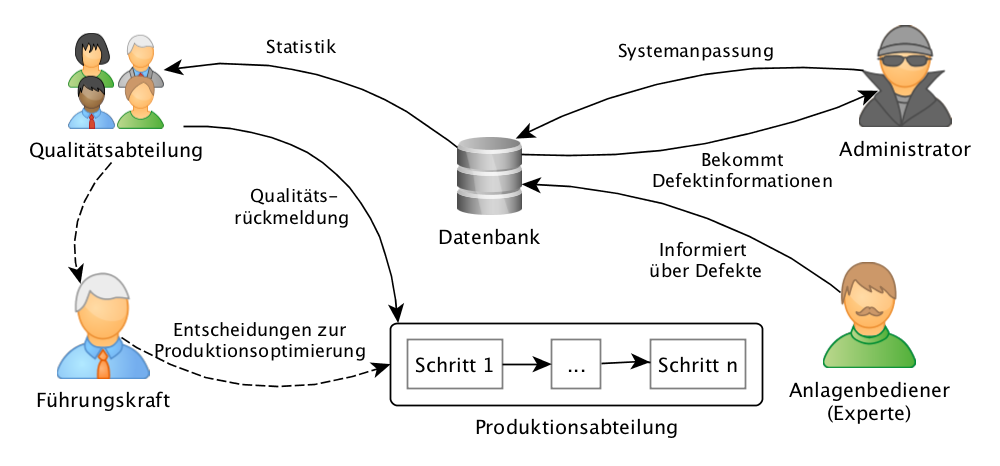
\includegraphics[width=0.95\textwidth]{images/dss_gebus.png}
	\caption{Die Struktur und die Informationsfl�sse im DSS, \cite[S.98]{gebus2009}}
	\label{dss_gebus}
\end{figure} 
Bei der Informationsrepr�sentation werden die Anlagenbilder benutzt. Die Autoren betonen, dass die Expertenschnittstelle einfach und intuitiv wie m�glich gehalten wurde, um die Dateneingabe zu einer allt�glichen T�tigkeit zu machen \cite[S.97]{gebus2009}. Im Hinblick auf die nicht-funktionalen Anforderungen werden beispielsweise Einstellungen und Maschinenbilder vom Administrator vorkonfiguriert und automatisch beim Hochfahren des Systems geladen. Die funktionalen Anforderungen umfassen die Erfassung einer St�rung durch die Auswahl des passenden Anlagebildes und das Markieren der betroffenen Stelle. Darauffolgend wird eine Vorlage mit m�glichen Ursachen zur Auswahl angezeigt. Zus�tzlich gibt es ein Feld zur Freitexteingabe, wenn die vorliegende St�rung im System noch nicht vorhanden ist \cite[S.99]{gebus2009}.\\
In der Evaluation haben sich folgende benutzerorientierte Kriterien f�r die weitere Systemverbesserung ergeben \cite[S.100]{gebus2009}:
\begin{itemize}
\item \textit{Usability (engl. Gebrauchstauglichkeit)}: wie einfach und intuitiv ist das System zu verwenden.
\item \textit{Usefulness (engl. N�tzlichkeit)}: wie n�tzlich ist das System f�r prim�re (Anlagenbediener) und sekund�re (z.B. Qualit�tsabteilung) Nutzer.
\item \textit{Usage (engl. Nutzung)}: inwiefern wird das System verwendet.
\end{itemize}
Wenn es um die Butzerinteraktion mit einem System geht, spielt Usability die zentrale Rolle. Gem�� ISO 9241-11 wird Usability durch folgende Aspekte definiert: Effektivit�t (wurde das Ziel erreicht), Effizienz (wie schnell wurde das Ziel erreicht) und Zufriedenheit (positive Erfahrung bei der Systemnutzung) \cite{iso9241}. In Bezug auf Usefulness ist eine interessante Ansicht in \cite{krug2014} gegeben. Steve Krug bezeichnet einen Gegenstand n�tzlich, wenn eine Person mit durchschnittlichen F�higkeiten herausfinden kann, wie dieser Gegenstand zu bedienen ist, um ein Ziel zu erreichen. Dabei soll der Aufwand kleiner als der Wert des Ziels sein \cite[S.9]{krug2014}.\\
Statistisch gesehen gab es in der betrachteten Testperiode 183 Anlagenausf�lle. Allerdings wurden nur 70 F�lle kommentiert, was die Nutzungsrate von 38\% ergibt. Laut Gebus und Leivisk{\"a} lag es daran, dass der Protoryp aus Usability-Perspektive nicht optimal war. Beispielsweise waren einige Elemente der Schnittstelle eher verwirrend. Nach den notwendigen Anpassungen konnte die Nutzungsrate fast bei 100\% erreicht werden. Hinsichtlich der N�tzlichkeit gab es positive Bewertungen. Es wurde festgestellt, dass die Umwandlung des Systems aus einer reinen Datensammlung �ber St�rungen zu einem Informationsaustauschsystem Vorteile f�r alle Nutzergruppen bringt. In der Abbildung \ref{dss_gebus} sieht man deutlich, dass die Informationen, die in der Datenbank gespeichert werden, von allen Beteiligten genutzt werden. Der Administrator kann mithilfe der Daten das System entsprechend anpassen. Die Qualit�tsabteilung setzt die Informationen zur Berichterstellung f�r die F�hrungskr�fte und die Produktion. Die Unternehmensf�hrung erh�lt ein umfangreicheres Bild �ber die Produktionslage und kann aufgrund dessen effizientere Entscheidungen bei der Produktionsoptimierung treffen. \\
Zusammenfassend l�sst sich sagen, dass die Entwicklung der Wissenstr�gerschnittstelle aus drei Phasen besteht. In der ersten Phase wird die Zielgruppe definiert. Im Hinblick auf die Zielgruppe werden die geeignete Informationsrepr�sentation sowie die funktionalen und nicht-funktionalen Anforderungen festgelegt. Die dritte Phase umfasst die Implementierung mit der darauffolgenden Evaluation, in dem die Schnittstelle nach drei Kriterien bewertet wird, n�mlich Usability, Usefulness und Usage.


\subsection{Datenerfassung aus dem Web}\label{subsec:webdaten}
Der Prozess der Webdatenerfassung umfasst die Datenextraktion aus den unstrukturierten bwz. semi-strukturierten Webdokumenten (z.B. eine Webseite oder eine E-Mail) und die Transformation der erfassten Daten in eine strukturierte Form f�r sp�tere Verwendung \cite[S.301]{ferrara2014}. Im Folgenden werden die allgemeinen Probleme bei der Erfassung der Webdaten angesprochen. Darauffolgend werden generelle Paradigmen der Datenerfassung erl�utert, n�mlich Baumparadigma, Web Wrapper und hybrides System.\\
Bei der Erfassung der Webdaten gibt es mehrere Faktoren, die ber�cksichtigt werden sollen. Ferrara et al identifizieren folgende Herausforderungen \cite[S.302]{ferrara2014}:
\newpage
\begin{itemize}
\item \textit{Automatisierungsgrad}: Die Erfassung der Webdaten soll oft von einem menschlichen Experten �berwacht werden, um die Genauigkeit der Daten zu gew�hrleisten.
\item \textit{Skalierbarkeit}: Bei den umfangreichen Webressourcen soll innerhalb k�rzer Zeit schnell eine gro�e Datenmenge bearbeitet werden.
\item \textit{Datenschutz}: Wenn es um die Erfassung der personenbezogenen Daten geht (bei sozialen Netzwerken wie Facebook), soll die Privatsph�re des Individuums nicht beeintr�chtigt werden.
\item \textit{�nderung der Ressourcenstruktur}: Die Struktur der Webressourcen �ndert sich oft. Die Datenerfassungsmethoden f�r das Web sollen eine gewisse Flexibilit�t besitzen, um weiterhin korrekt zu funktionieren.
\item \textit{Trainingsdaten}: Bei der Einsetzung des maschinellen Lernen ist eine ausreichende Trainingsmenge an Webseiten erforderlich, die manuell vorbereitet wird. Dies ist eine schwierige und fehleranf�llige Aufgabe.
\end{itemize}
Das Baumparadigma nutzt die Baumstruktur einer Webseite aus, um die gew�nschten Daten zu erfassen. Dabei handelt es sich um Dokumente, die in \acf{HTML} beschrieben sind. Eine HTML-Seite wird als \acf{DOM}\footnote{https://www.w3.org/DOM} definiert. Die Idee vom DOM besteht darin, dass die HTML-Webseite ein Baum darstellt, der mittels HTML-Tags (z.B. Button-Tag) ausgezeichnet wird. Tags k�nnen weitere Tags beinhalten und bilden somit eine hierarchische Struktur. Diese hierarchische Baumstruktur erm�glicht effiziente Datensuche in einer HTML-Seite \cite[S.303]{ferrara2014}.\\
Da HTML ein Dialekt von \acf{XML} ist, kann \acf{XPath}\footnote{https://www.w3.org/TR/xpath} f�r die Navigation in DOM eingesetzt werden. In einem XPath-Ausdruck k�nnen beliebige Elemente einer HTML-Webseite ausgew�hlt werden. In Abbildung \ref{xpath} werden zwei Beispiele dargestellt. Im ersten Fall (A) wird genau ein Element (die erste Zelle in der ersten Reihe) ausgew�hlt. Im Beispiel (B) werden mehrere Elemente (alle Zellen der zweiten Reihe) angesprochen \cite[S.303]{ferrara2014}.
\begin{figure}[H] 
	\centering
	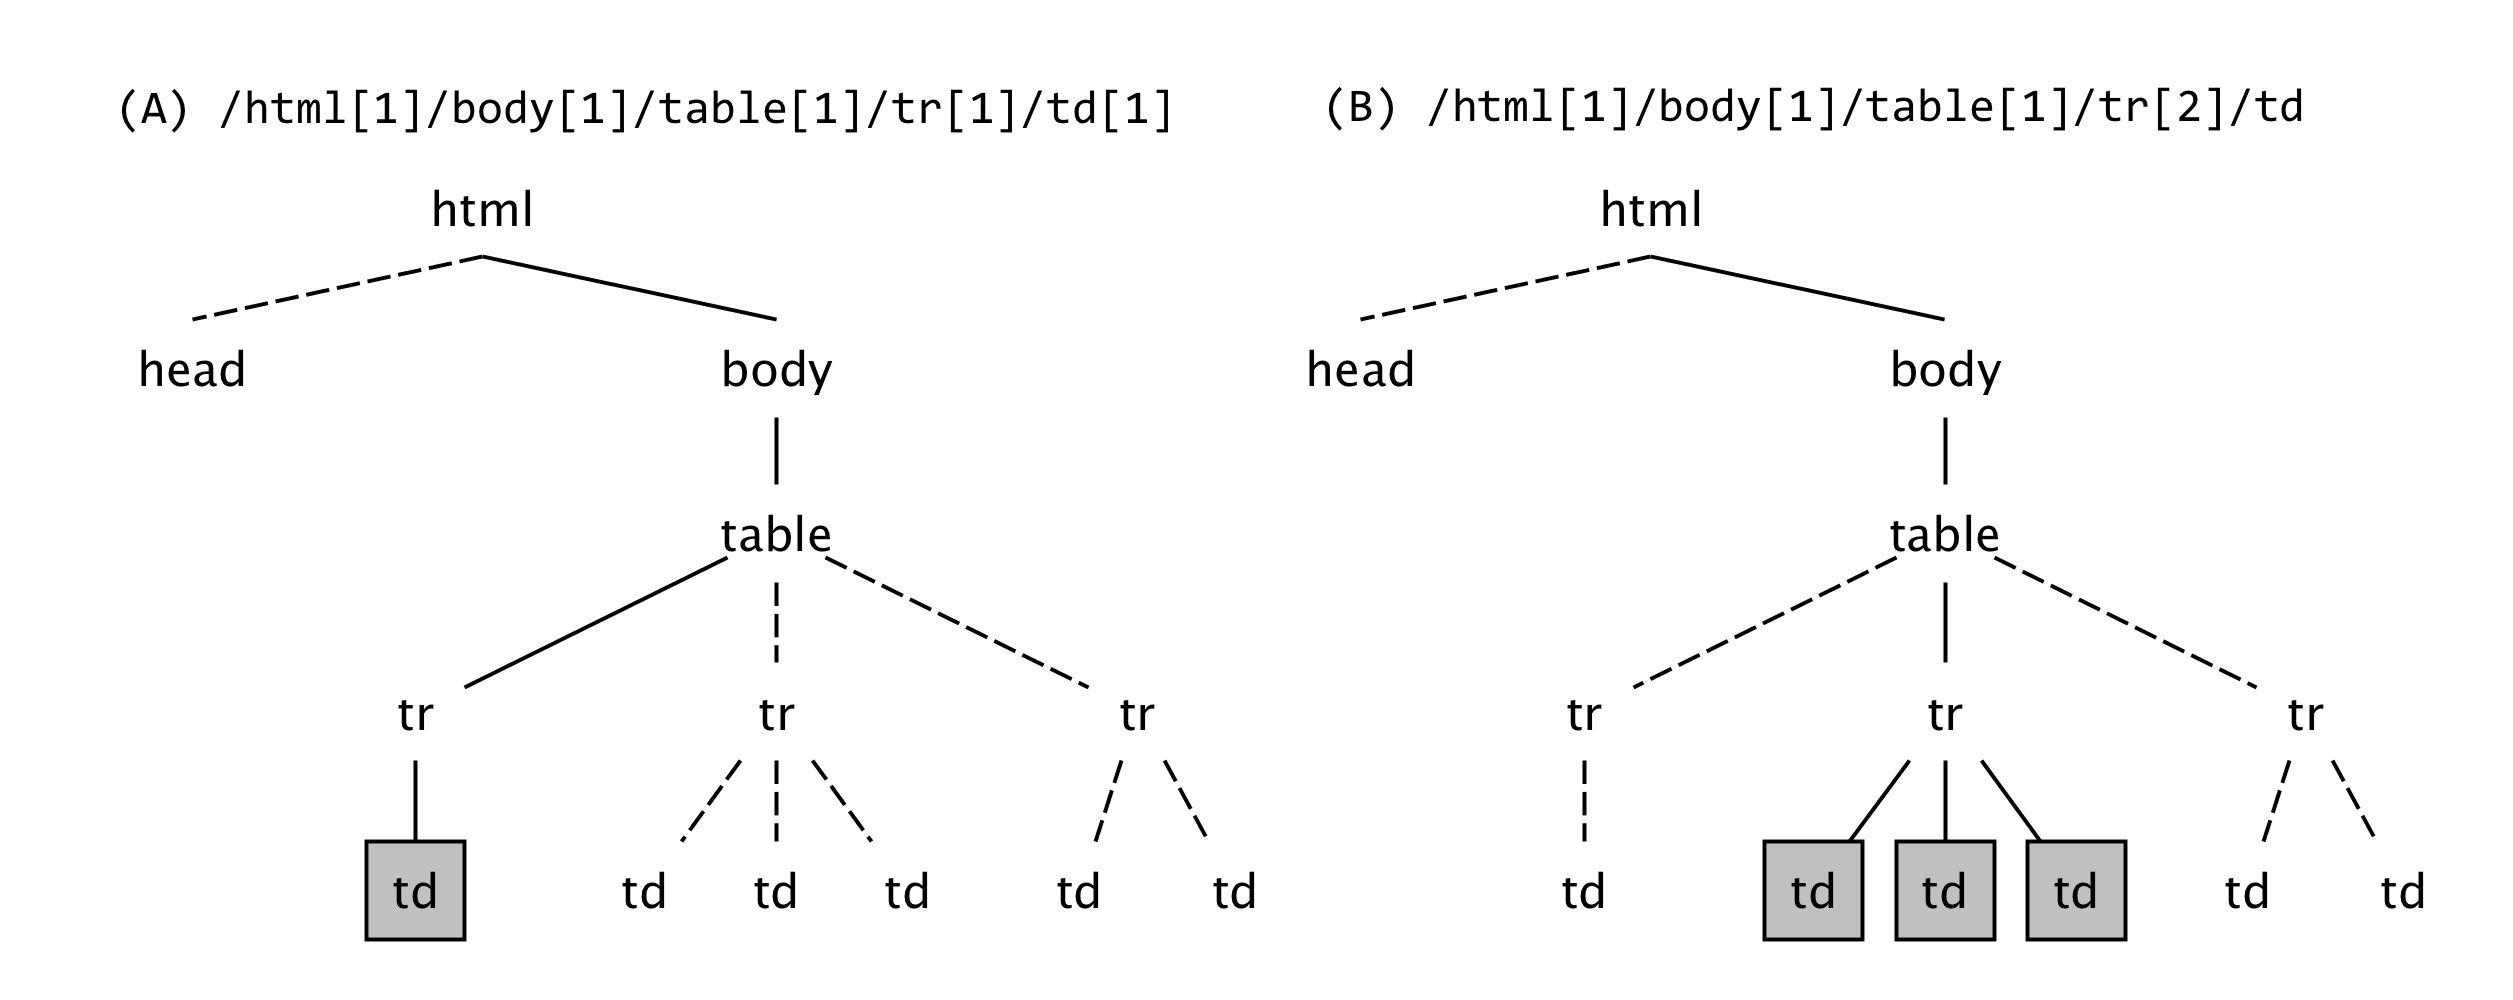
\includegraphics[width=1.0\textwidth]{images/xpath.png}
	\caption{XPath im Dokumentenbaum, \cite[S.304]{ferrara2014}}
	\label{xpath}
\end{figure} 
Der Hauptnachteil von XPath besteht darin, dass XPath-Ausdr�cke strikt an der DOM-Struktur gebunden sind. Wenn eine �nderung im DOM stattfindet, funktioniert der von der �nderung betroffene Ausdruck nicht mehr. Aus diesem Grund m�ssen die XPath-Ausdr�cke nach jeder Ver�nderung der HTML-Webseite manuell angepasst werden. In Bezug auf dieses Problem wurde im letzten Release von XPath\footnote{https://www.w3.org/TR/xpath20} relative XPath-Ausdr�cke eingef�hrt \cite[S.304]{ferrara2014}.\\
Ein weiterer Ansatz, die Webdaten zu erfassen, stellt ein Web Wrapper dar. Das Web Wrapper umfasst in der Regel einen oder mehreren Algorithmen, die zur Datenerfassung aus den Webdokumenten eingesetzt werden. Anschlie�end werden die erfassten Daten in eine strukturierte Form transformiert und f�r weitere Nutzung gespeichert. Ein Web Wrapper umfasst folgende Schritte \cite[S.305]{ferrara2014}:
\begin{itemize}
\item[1.]\textit{Generierung}: Definition des Wrappers.
\item[2.]\textit{Ausf�hrung}: Datenerfassung mithilfe des Wrappers.
\item[3.]\textit{Wartung}: Anpassung des Wrappers bei der �nderung der DOM-Struktur.
\end{itemize}
Nach Ferrara et al kann ein Web Wrapper mittels folgender Ans�tze generiert und ausgef�hrt werden \cite[S.306]{ferrara2014}:
\begin{itemize}
\item \textit{Regul�re Ausdr�cke}: Daten werden gem�� Regeln (expressions) gewonnen. Im Rahmen dieser Arbeit wird es im Weiteren aus regul�re Ausdr�cke beschr�nkt.
\item \textit{Logikbasierter Ansatz}: Zur Datenerfassung wird eine Wrapper Programmiersprache eingesetzt (wrapper programming language).
\item \textit{Baumbasierter Ansatz}: Dabei wird die Annahme getroffen, dass bestimmte Bereiche im DOM generell f�r Daten zust�ndig sind. Die Identifikation und Datenextraktion aus diesen Bereichen ist der Gegenstand des baumbasierten Ansatzes.  
\item \textit{Maschinelles Lernen}: Daten werden mithilfe eines Lernalgorithmus und einer Trainingsmenge erfasst.
\end{itemize} 
Regul�re Ausdr�cke erm�glichen die Erkennung von Patterns in der unstrukturierten bzw. semi-strukturierten Dokumenten unter Verwendung der Regeln, die z.B. in Form von Wortgrenzen oder HTML-Tags definiert werden. Der Vorteil der regul�ren Ausdr�cken besteht in der M�glichkeit, beliebiges Element auf einer Webseite anzusprechen. Au�erdem bieten einige Implementierungen ein grafisches Benutzerinterface, sodass der Benutzer die Elemente auf einfache Weise ausw�hlen kann. Die Regeln werden dann automatisch generiert. Eine m�gliche Umsetzung des Wrappers wird in \cite{sahuguet1999} mit W4F vorgestellt. Das Tool verf�gt �ber eine Hilfsmethode, die den Benutzer bei der Auswahl der Elementen unterst�tzt. Auf Basis der ausgew�hlten Elementen werden die Regeln erstellt. Allerdings sind die Regeln in Bezug auf DOM-�nderungen nicht flexibel und k�nnen sehr schnell verletzt werden \cite[S.306]{ferrara2014}.\\
In der dritten Phase geht es um die Anpassung des Web Wrappers im Hinblick auf die Ver�nderungen der DOM-Struktur. Die Anpassung erfolgt entweder manuell oder in gewisser Weise automatisiert. Ferrara et al betonen, dass der Automatisierungsgrad der Wartung besonders kritisch ist \cite[S.308]{ferrara2014}. Bei einer kleinen Dokumentenanzahl ist die manuelle Anpassung noch akzeptabel. Allerdings ist die manuelle Wartung bei einer gro�en Menge der Dokumente nicht mehr denkbar.\\
Ein Beispiel der automatisierter Wrapper-Wartung wird in \cite{meng2003} mit dem System namens SG-WRAM (Schema-Guided Wrapper Maintenance for Web-Data Extraction) vorgestellt. Die Architektur vom SG-WRAM wird in der Abbildung \ref{wram} dargestellt.
\begin{figure}[H] 
	\centering
	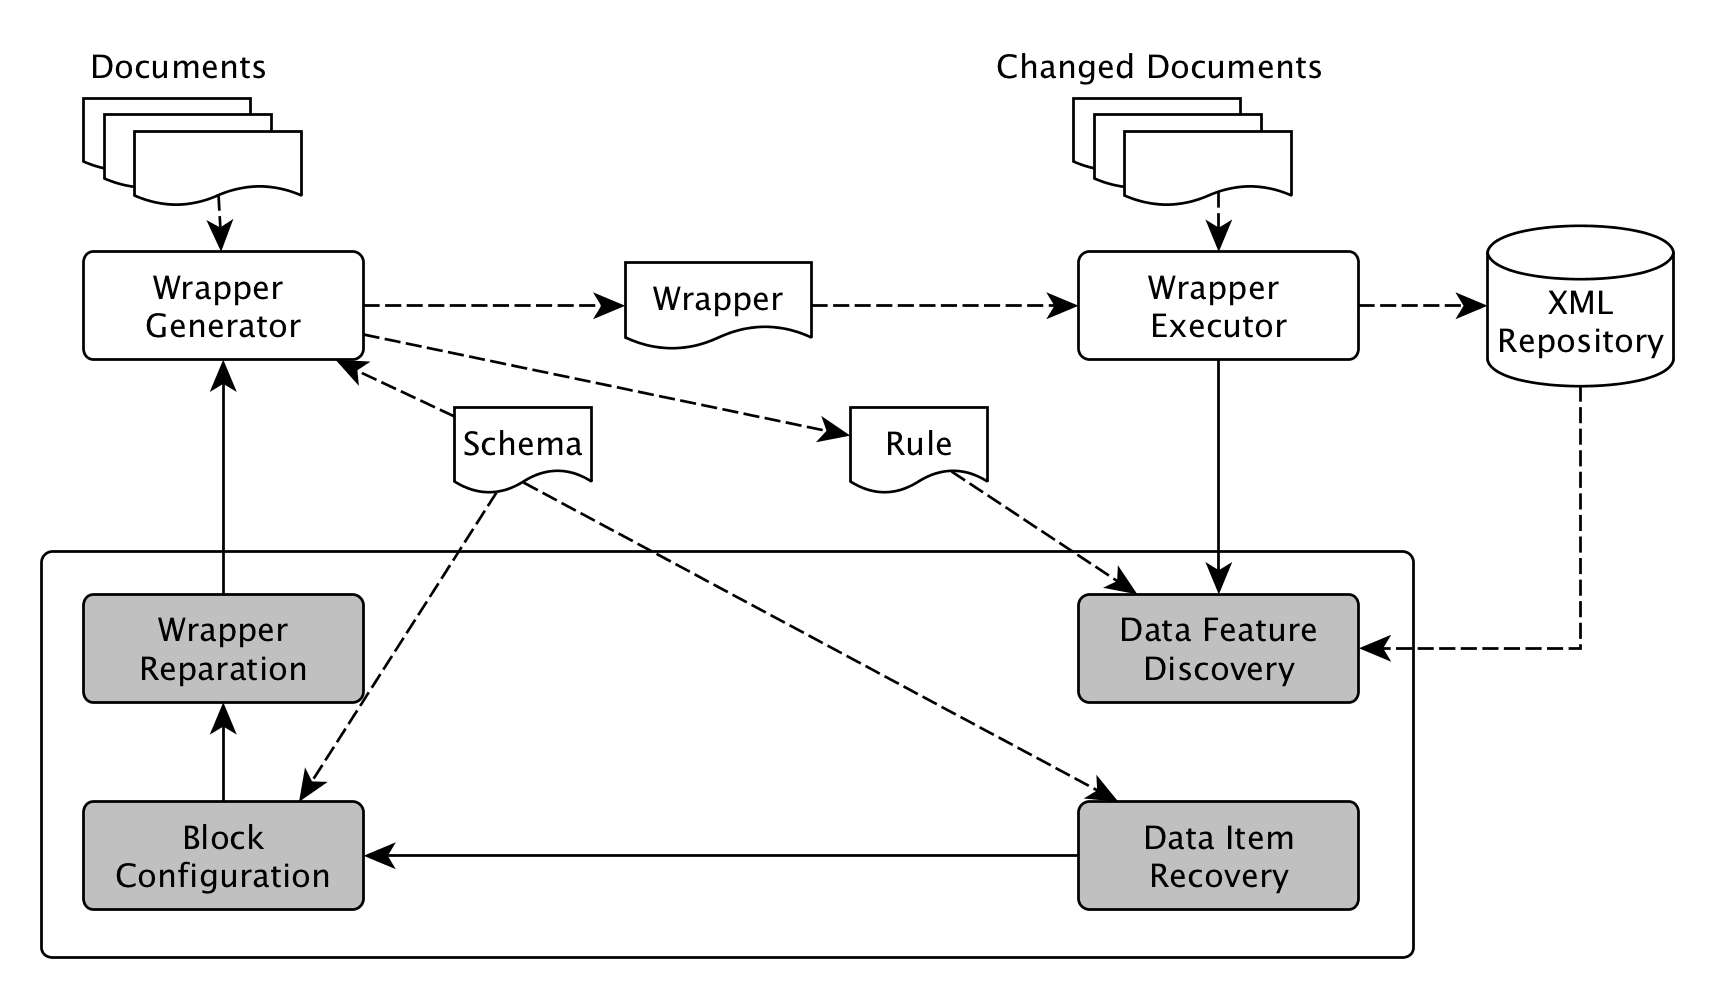
\includegraphics[width=0.95\textwidth]{images/wram.png}
	\caption{Die Architektur vom SG-WRAM, \cite[S.2]{meng2003}}
	\label{wram}
\end{figure} 
Im ersten Schritt werden die HTML-Seite, XML-Schemata und das Mapping zwischen diesen beim Wrapper-Generator eingegeben. XML-Schema wird in \acf{DTD} beschrieben. Darauffolgend generiert das System die Regeln (Wrapper) f�r die gegebene Webseite, um die Daten zu erfassen und in einer XML-Datei gem�� der DTD-Datei zu speichern. Neben der Datenextraktion werden zus�tzlich die Probleme bei der Extraktion erfasst, um ein Wiederherstellungsprotokoll f�r die fehlgeschlagenen Regeln zu erzeugen. Wenn das Protokoll die Fehler beseitigt, wird die Datenerfassung fortgesetzt. Beim Fehlschlag werden Warnungen und Benachrichtigungen angezeigt, dass die Regeln nicht mehr funktionieren. In diesem Fall sollen die Regeln manuell von einem Experten angepasst werden \cite[S.308]{ferrara2014}.\\
Als ein Ausblick wird ein hybrides System der Webdatenerfassung angesprochen. Ein Beispiel des hybriden Ansatzes stellt RoadRunner von \cite{crescenzi2001} dar. RoadRunner kann sowohl mit der Trainingsmenge von einem Nutzer als auch mit selbst erstellten Trainingsdaten ausgef�hrt werden. Das Verfahren arbeitet gleichzeitig mit zwei HTML-Seiten und analysiert die Gemeinsamkeiten und die Unterschiede zwischen diesen Seiten, um die Patterns zu finden. Allgemein kann das Verfahren die Daten aus beliebiger Quelle erfassen, die mindestens zwei Seiten mit �hnlicher Struktur sind. Da Webseiten normalerweise dynamisch auf Basis eines Templates generiert werden, befinden sich relevante Daten in gleichen oder �hnlichen Bereichen \cite[S.309]{ferrara2014}.
\subsection{Maschinelles Lernen beim Wissenserwerb}
Eine weitere M�glichkeit zur Automatisierung des Wissenserwerbs stellen die Methoden des maschinellen Lernens dar. In der Literatur gibt es eine Reihe der Ans�zte, die sich damit besch�ftigen (z.B. \cite{castro2001} und \cite{webb1996}). Trotz der Unterschieden in der Umsetzung gibt es eine entscheidende Gemeinsamkeit. Beide Methoden basieren auf der Zusammenarbeit zwischen dem Experten und dem Lernalgorithmus. Im Folgenden wird der Ansatz von \cite{castro2001} genauer betrachtet.\\
In der Arbeit von \cite{castro2001} handelt es sich um die Anwendung des maschinellen Lernens bei der Erfassung des Expertenwissens im Medizinbereich. Das Konzept der Wissensbasiserweiterung orientiert sich an \cite{tecuci1992} und besteht darin, dass anfangs eine initiale Wissensbasis gebaut und inkrementell verbessert wird, indem der Experte die Fragen vom System beantwortet. Bei der Erstellung der Fragen wird ein Lernalgorithmus verwendet. Die Idee des Lernalgorithmus besteht in der Erschlie�ung des allgemeinen Expertenwissens aus den Trainingsdaten der Schlussfolgerungen eines Experten.\\
Der Kern des Lernalgorithmus besteht aus dem induktiven Lernen und dem generischen Algorithmus von \cite{castro1999}, der auf der Fuzzylogik basiert ist. Bei der Induktion handelt es sich um das Erschlie�en der allgemeinen Schlussfolgerungen aus den Einzelf�llen. Die Fuzzylogik besch�ftigt sich mit den graduellen Aussagen, die nicht eindeutig falsch oder wahr bezeichnet werden k�nnen. Diese Aussagen werden mithilfe der vagen Pr�dikaten beschrieben. Ein typisches Beispiel ist das Pr�dikat \glqq{}gro�\grqq{}. Eine 1,80 m gro�e Person wird als \glqq{}gro�\grqq{} bezeichnet, w�hrend eine 1,75 m Person ist nicht genau so \glqq{}gro�\grqq{}, aber auch nicht \glqq{}klein\grqq{} ist \cite[S.27]{beierle2014}.\\
Der Lernalgorithmus ist wie folgt aufgebaut \cite[S.316]{castro2001}:
\begin{itemize}
\item[1.] Eingabe der Trainingsdaten.
\item[2.] Entfernen des Rausches aus den Trainingsdaten.
\item[3.] Ermittlung der Genen, die sich nicht �ndern k�nnen.
\item[4.] Ermittlung der Menge der initialen Regeln mithilfe des Algorithmus von \cite{castro1999}.
\item[5.] Anwendung des Algorithmus von \cite{castro1999} zur Ermittlung der Menge der Regeln, die das allgemeine Expertenwissen aus der Trainingsmenge beschreiben.
\item[6.] Ausschluss der Regeln, die ein Teil anderer Regeln sind.
\item[7.] Ende.
\end{itemize}
Aufgrund der hohen Komplexit�t und des spezifischen Anwendungsbereichs des Algorithmus wird es im Weiteren auf den ersten Schritt beschr�nkt, der das grundlegende Verst�ndnis �ber den Algorithmus liefert.\\
Als Erstes definieren Castro et al die Wissensrepr�sentation. Es werden folgende Informationstypen unterschieden \cite[S.309]{castro2001}:
\begin{itemize}
\item \textit{Numerische Information}, die aus einer empirischen Beobachtung stammt und als eine Beispielmenge von Input-Output-Beziehungen erfasst wird.
\item \textit{Sprachinformation}, die von einem Experten stammt und in Form von IF-THEN-Regeln beschrieben wird.
\end{itemize}
Die Trainingsmenge wird folgenderma�en definiert (siehe Formeln \ref{eq:trainingsmenge} und \ref{eq:training}):
\begin{equation}
	\theta = \lbrace e_1 \dots e_m \rbrace
	\label{eq:trainingsmenge}
\end{equation}
\begin{equation}
	e_i = ((x_{i0}, \dots , x_{in}), y_j)
	\label{eq:training}
\end{equation}
wobei:
\begin{itemize}
\item[\( \theta \)] = Trainingsmenge;
\item[\( e_i \)] = Schlussfolgerung
\item[\( m \)] = Anzahl der vorhandenen Schlussfolgerungen;
\item[\( n \)] = Anzahl der Input-Variablen in der Schlussfolgerung;
\item[\( x_{in} \)] = Input-Variablen
\item[\( y_j \)] = Output-Wert (Expertenschlussfolgerung).
\end{itemize}
Die Output-Werte nach der Formel \ref{eq:training} stellen die Teilmenge des kartesischen Produkts aller Input- und Output-Werten \(X^n \times Y \) dar. Das Ziel ist die Approximation der Funktion \( \Omega: X^n \rightarrow Y \) durch die Ermittlung von Fuzzy-IF-THEN-Regeln, um das allgemeine Expertenwissen aus der Trainingsmenge zu erschlie�en. Fuzzy-IF-THEN-Regel wird wie folgt definiert (siehe Formel \ref{eq:fuzzy-regel}):
\begin{equation}
	R_j : \mbox{ IF } X \mbox{ is } E \mbox{ THEN } Y \mbox{ is } y_i 
	\label{eq:fuzzy-regel}
\end{equation}
wobei:
\begin{itemize}
\item[\( R_j \)] = eine Regel
\item[\( X \)] = Menge der Variablen in den Schlussfolgerungen;
\item[\( E \)] = Teilmengen der Fuzzy-Labels
\item[\( Y \)] = Expertenschlussfolgerung
\end{itemize}
Castro et al treffen die Annahmen, dass die Teilmengen der Fuzzy-Labels \( E \) aus einer endlichen Menge der Labels $\mathcal{L}$ entnommen sind (siehe Formel \ref{eq:fuzzy-labels}):
\begin{equation}
	\mathcal{L} = \lbrace L_{i1}, \dots , L_{ik} \rbrace
	\label{eq:fuzzy-labels}
\end{equation}
Dabei ist \( k \) die Anzahl der Labels und \( E_i \) ist eine Expertenschlussfolgerung, die ein Element der Funktionsmenge \( \mathcal{P}(\mathcal{L}_i) \), oder zusammenfassend \( E_i \in \mathcal{P}(\mathcal{L}_i) \).\\
Das Ergebnis der Durchf�hrung des Algorithmus ist eine Menge der Regeln, die bei der Erstellung der Fragen verwendet werden. Dabei kann die Differenzstrategie eingesetzt werden \cite[S.317]{castro2001}. Bei der Differenzstrategie werden die Regeln gesucht, die zu einem Konflikt f�hren, wenn sie gleichzeitig angewandt werden. Um den Konflikt zu l�sen, kann der Experte eine neue Variable zulassen. Alternativ kann der Experte eine neue Meta-Regel definieren, wie z.B wenn \( R_i \) und \( R_j \) sich widersprechen, soll \( R_i \) bevorzugt werden, da es die allgemeinere Klasse repr�sentiert \cite[S.318]{castro2001}.
\newpage
\section{Implementierung der Wissensewerbskomponente}\label{sec:Implementierung}
Nachdem die theoretischen Grundlagen von der Wissenserfassungskomponente betrachtet wurden, geht es im vorliegenden Kapitel um die praktische Umsetzung am Beispiel von \textit{PaaSfinder}\footnote{https://paasfinder.org}. Zuerst wird der Zweck und das Ziel von \textit{PaaSfinder} beschrieben. Als n�chstes werden geeignete Datenerfassungsmethoden im Rahmen von \textit{PaaSfinder} ausgew�hlt und implementiert.
\subsection{Allgemein zum \textit{PaaSfinder}}
\begin{itemize}
\item der Zweck vom \textit{PaaSfinder}
\item OpenSource und Github
\item Struktur des Dateneintrags: JSON, Attribute, Bedeutung 
\item Problem - Git-Repository runterladen, JSON �ndern und pushen 
\end{itemize}

\subsection{Wissenstr�gerschnittstelle}\label{sec:Wissenstr�gerschnittstelle}
Als erster Schnitt in der Automatisierung der Datenerfassung bei \textit{PaaSfinder} wird eine Schnittstele zur Dateneingabe entwickelt (Wissenstr�gerschnittstelle). Mithilfe der Schnittstelle soll die Aktualisierung eines bestehenden Profils erm�glicht werden. Das Anlegen oder das L�schen eines Profils liegt nicht im Anwendungsbereich der Schnittstelle. Der Ablauf wird in Abbildung \ref{fig:update-allgemein} veranschaulicht.
\begin{figure}[H] 
	\centering
	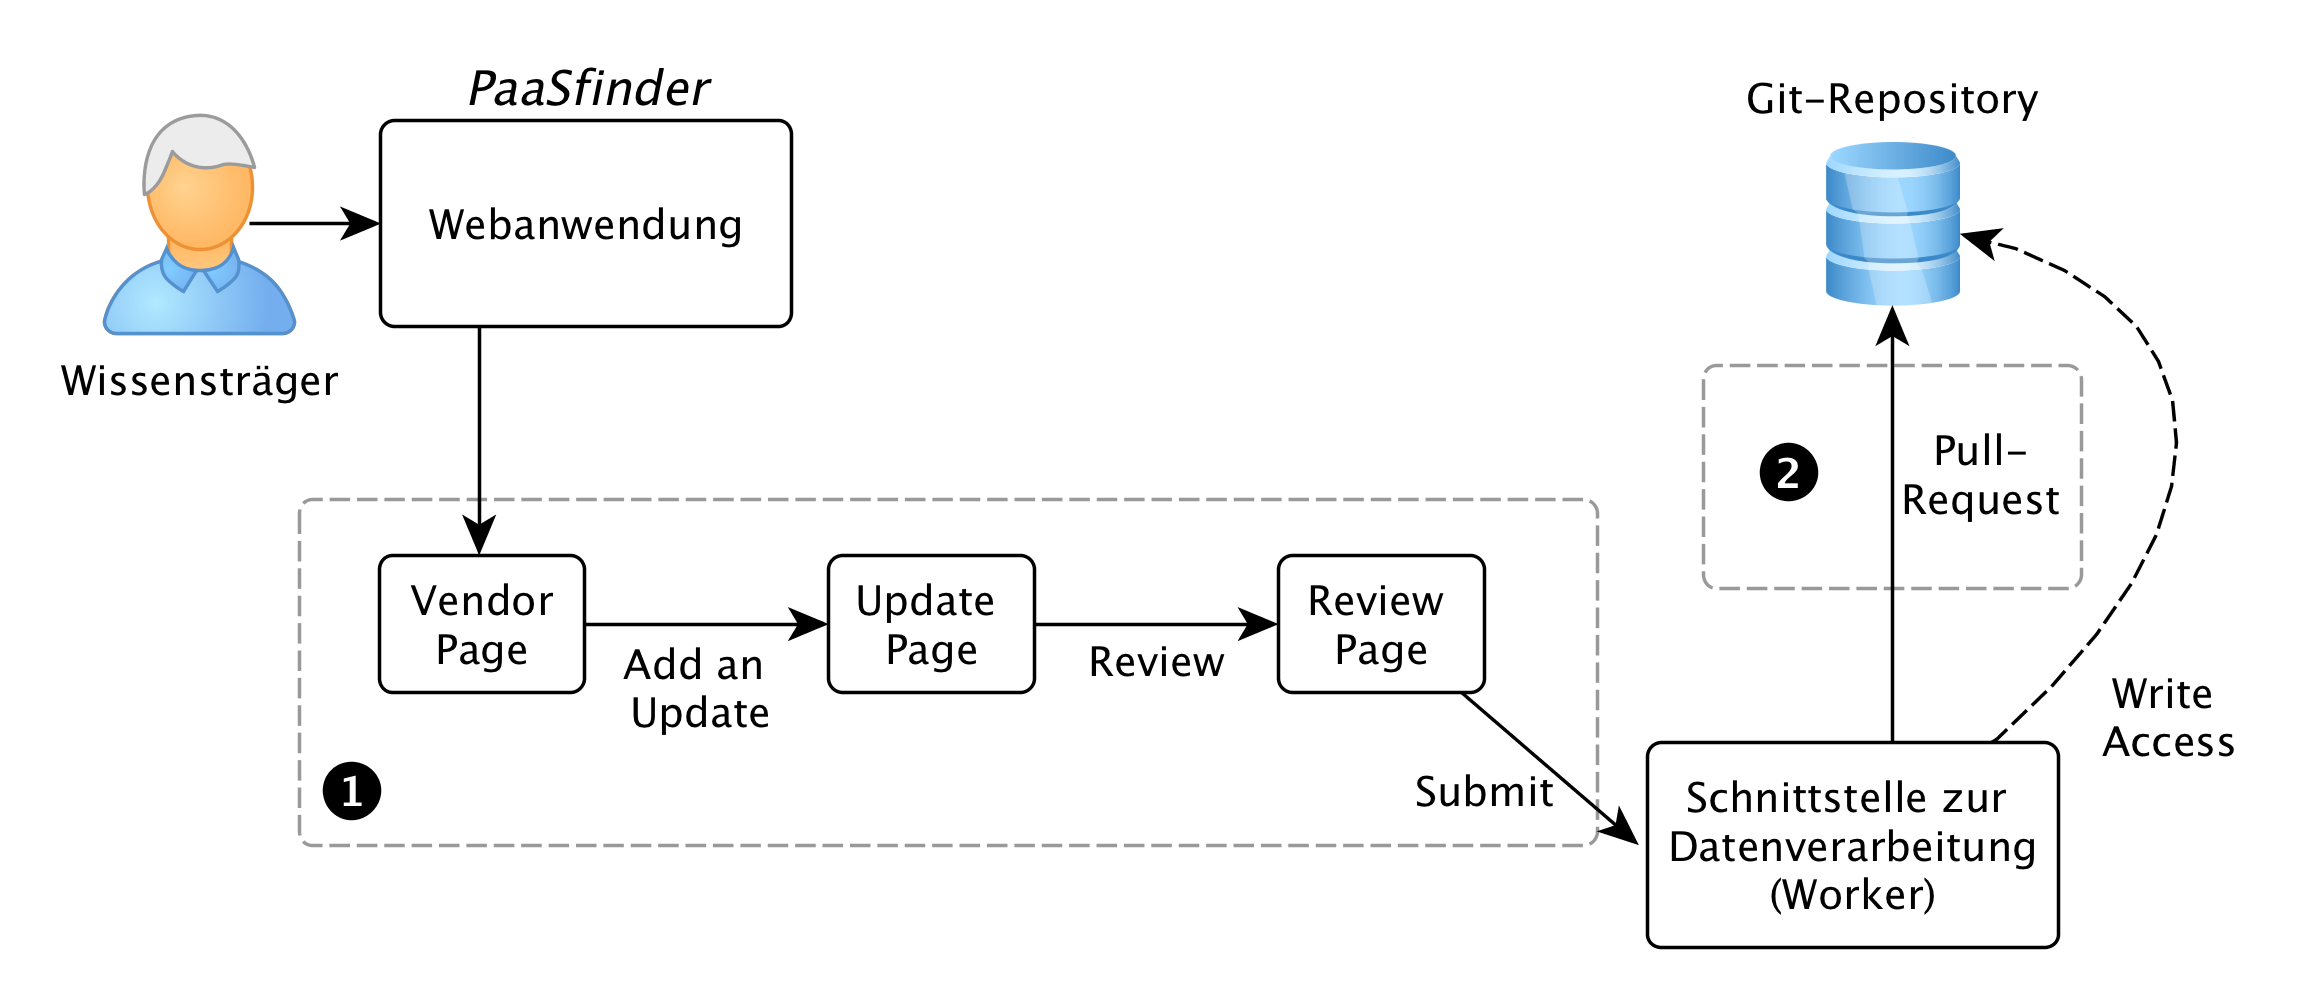
\includegraphics[width=1.0\textwidth]{images/update.png}
	\caption{Profilaktualisierung mittels Wissenstr�gerschnittstelle}
	\label{fig:update-allgemein}
\end{figure}
Der Ablauf in Abbildung \ref{fig:update-allgemein} l�sst sich in zwei Schritte aufteilen. Dieser Abschnitt besch�ftigt sich mit dem ersten Schritt, der die Daten von einem Wissenstr�ger entgegennimmt, zusammenfasst und abschickt. Die Verarbeitung dieser Daten erfolgt im zweiten Schritt, der im n�chsten Abschnitt besprochen wird. Allgemein besteht der erste Schritt aus folgenden Aktionen:
\begin{enumerate}
\item \textit{Profilauswahl} (Vendor Page)
\item \textit{Aktualisieren} des Profils (Update Page)
\item \textit{�berpr�fung} der Daten (Review Page)
\item \textit{Absenden} der Daten (Sumbit)
\end{enumerate}
Der gesamte Prozess l�sst sich in Abbildung \ref{fig:activity} als ein Aktivit�tsdiagramm darstellen. Die verwendete Notation entspricht dem UML-Standard 2.5 \cite[S.398]{uml2}. Es werden Knoten (Rechteck) f�r Aktivit�ten und Kanten (Pfeile) f�r Verbindungen verwendet. Bei den Verbindungen werden Kontrollfluss- und Datenflussverbindungen unterschieden. Im Fall einer Datenflussverbindung gibt es ein Ein- und der Ausgabe-Pin (kleiner Quadrat) am Anfang oder am Ende des Pfeils. Im vorliegenden Fall werden noch Fallunterscheidungen verwendet, die durch eine Raute gekennzeichnet sind.
\begin{figure}[H] 
	\centering
	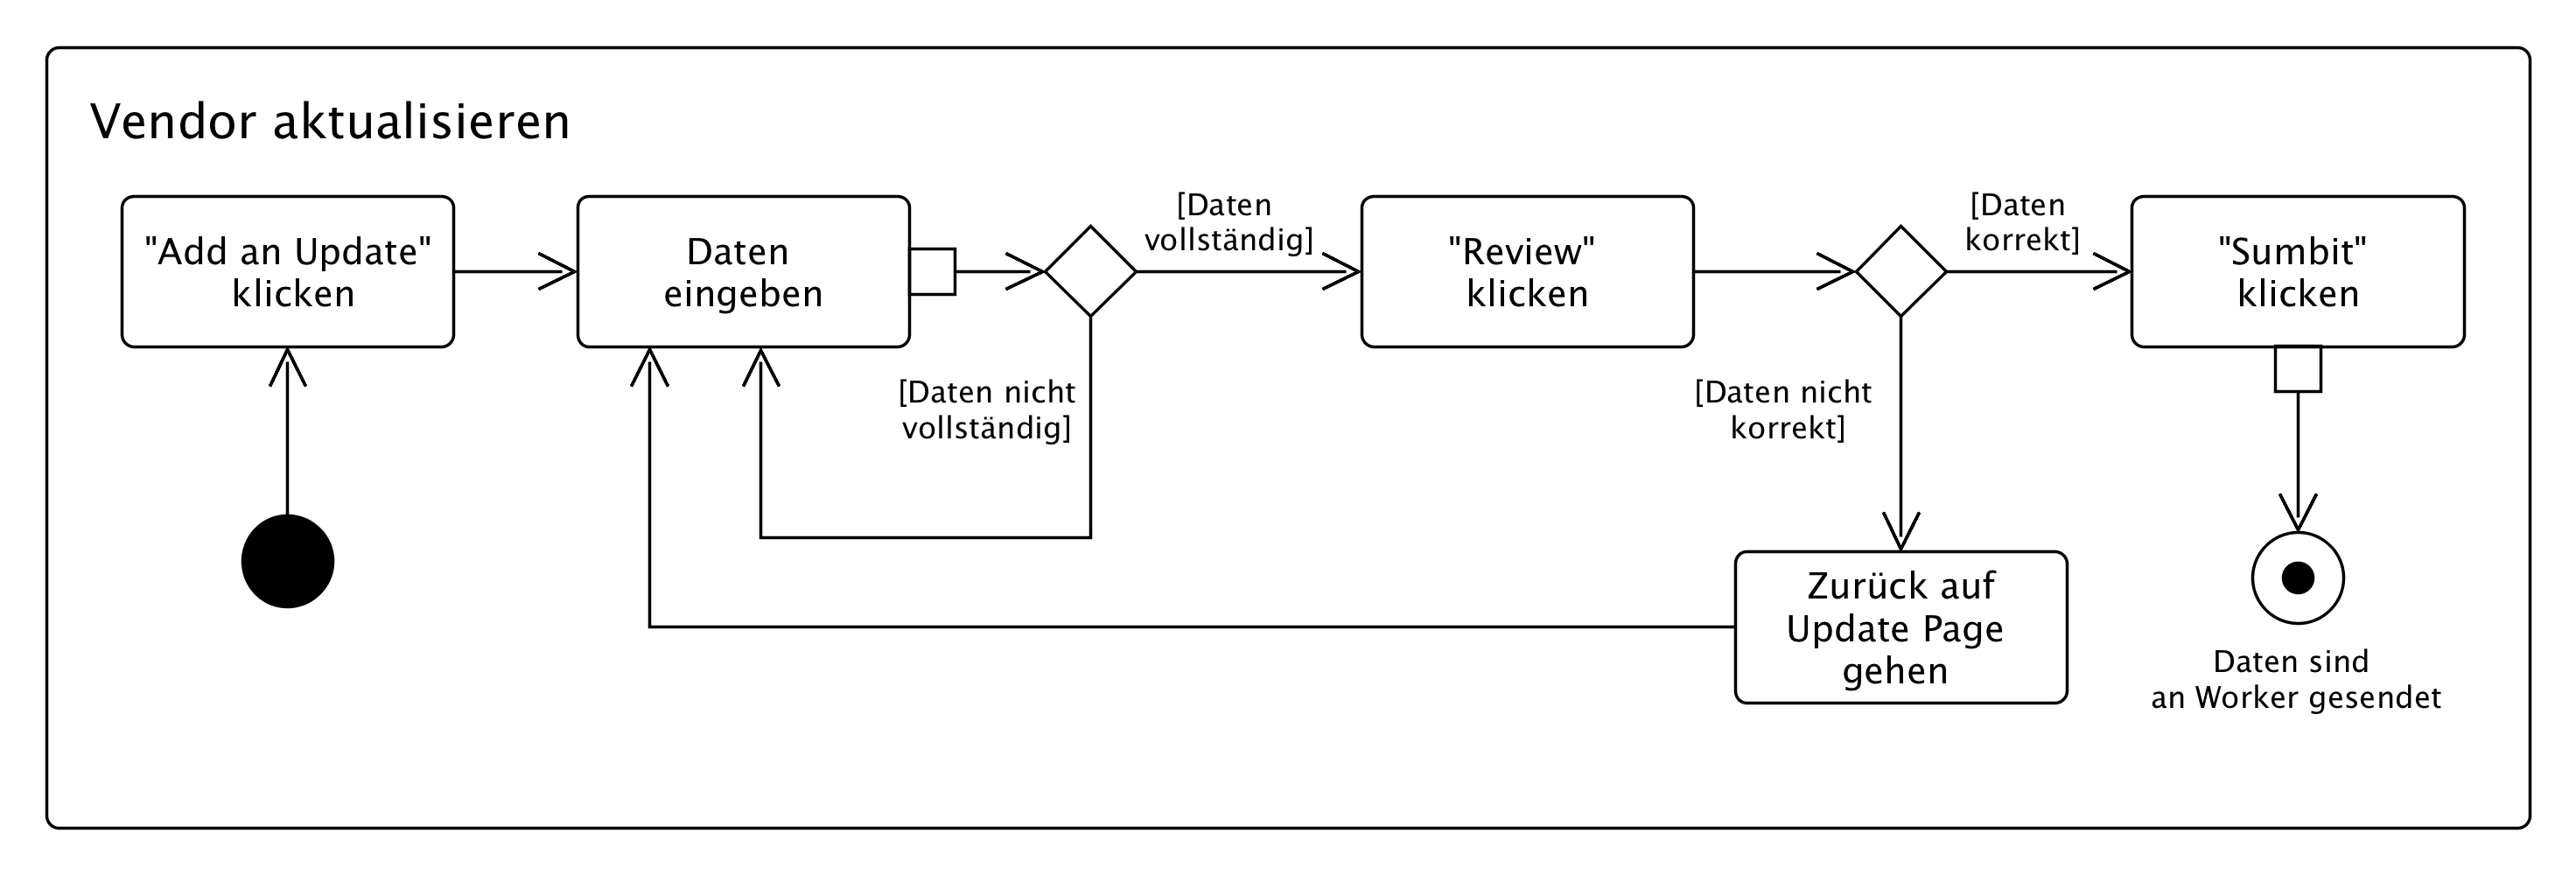
\includegraphics[width=1.0\textwidth]{images/activity.png}
	\caption{Aktivit�tsdiagramm der Aktualisierung des PaaS-Profils}
	\label{fig:activity}
\end{figure}
Ausgehend von einer Vendor Page wird der Ablauf mit \glqq{}Add an Update\grqq{} gestartet. Als n�chstes werden die Daten eingegeben. Wenn das Profil aus Sicht des Wissenstr�gers vollst�ndig ist, wird auf \glqq{}Review\grqq{} geklickt. Sonst wird der Schritt der Dateneingabe wiederholt. Falls der \glqq{}Review\grqq{}-Button geklickt wurde, gelangt man zur Review Page. Hier k�nnen die Daten �berpr�ft werden. Wenn die Daten korrekt sind, kann das aktualisierte Profil mit dem Klick auf \glqq{}Submit\grqq{} an den Worker gesendet werden. Anderenfalls kann der Wissenstr�ger zur�ck zur Dateneingabe gehen und die Daten �berarbeiten. In jedem Zeitpunkt besteht die M�glichkeit, den Vorgang abzubrechen, indem das Browserfenster geschlossen wird. Die Daten werden nur dann gesendet, wenn der \glqq{}Submit\grqq{}-Button auf der Review Page geklickt wird. Im weiteren Verlauf wird die Implementierung der Page und Review Page beschrieben.\\
Die Update Page umfasst zwei Aspekte. Erstens sollen die Profildaten f�r den Wissenstr�ger geeignet dargestellt werden Zweitens soll die Eingabe der Daten erm�glicht werden. Au�erdem sollen die �nderungen am Profil dynamisch zwischengespeichert werden. Das ist eine herausfordernde Aufgabe, da ein Profil, abgesehen von allgemeinen Eigenschaften (z.B. \glqq{}name\grqq{}), aus komplexen und teils verschachtelten Datentypen besteht. In Abbildung \ref{fig:profil} wird das am Beispiel von \glqq{}runtimes\grqq{} (Laufzeitumgehungen) gezeigt. Farbe gelb steht dabei f�r ein Objekt, grau f�r eine Liste und wei� f�r ein String (Zeichenkette). Hier umfasst ein Profil (\glqq{}vendor\grqq{}) eine Liste von \glqq{}runtimes\grqq{}. \glqq{}Runtime\grqq{} besteht wiederum aus \glqq{}language\grqq{} und \glqq{}versions\grqq{}.
\begin{figure}[H] 
	\centering
	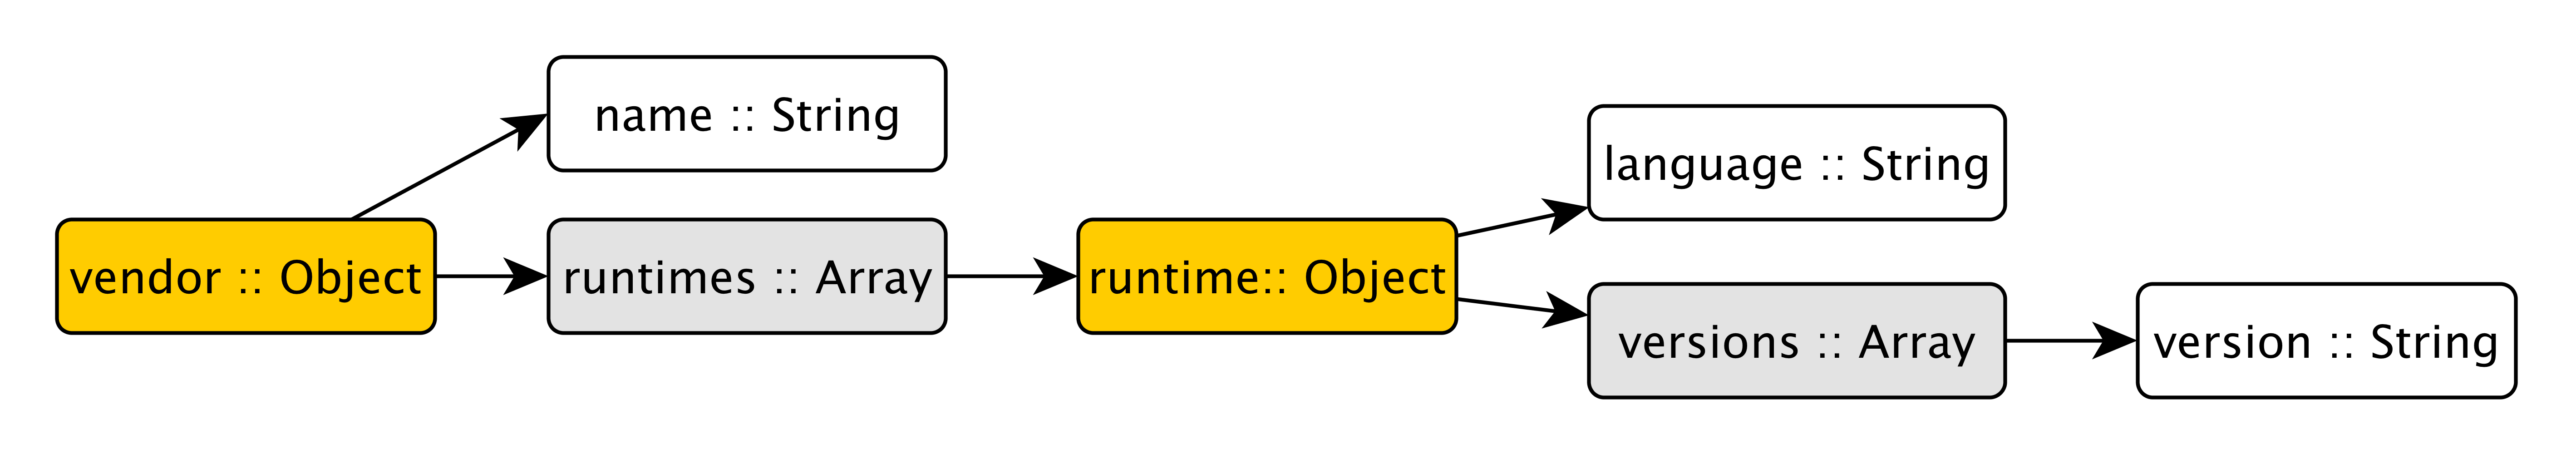
\includegraphics[width=1.0\textwidth]{images/vendor.png}
	\caption{Komplexe Datentypen im PaaS-Profil}
	\label{fig:profil}
\end{figure}
Um diese Aufgabe zu l�sen, werden die Daten in zwei Richtungen gebunden (two-way data binding). Zu diesem Zweck wird ein Open-Source Framework Knockout.js\footnote{http://knockoutjs.com} eingesetzt. Knockout.js ist eine JavaScript Bibliothek zur Erstellung dynamischer Webseiten. Das Framework basiert auf \ac{MVVM} Entwurfsmuster\footnote{http://knockoutjs.com/documentation/observables.html}:
\begin{itemize}
\item \textit{Model}: Daten, die unabh�ngig auf einem Server liegen (hier: verf�gbare PaaS-Profile)
\item \textit{ViewModel}: Programmcode der Daten und Operationen auf der Benutzerschnittstelle (hier: JavaScript Klasse f�r PaaS-Profil (Modell))
\item \textit{View}: Benutzerschnittstelle, die den Zustand von ViewModel abbildet und bei Benutzeraktionen aktualisiert (hier: Update Page)
\end{itemize}
Als erstes werden die f�r das Modell erforderliche Daten �ber \textit{PaaSfinder}-\acs{API}\footnote{https://paasfinder.org/api/vendors/} geholt und das Modell initialisiert. Da das Modell komplexe Datentypen umfasst, sind explizite JavaScript Klassen n�tig. Beispielsweise gibt es f�r \glqq{}runtime\grqq{} und \glqq{}version\grqq{} jeweils eigene Klassen mit unterschiedlichem Verhalten. Die Klasse \glqq{}runtime\grqq{} beinhaltet z.B. die Methode zum Hinzuf�gen neuer Version. Nachdem das Modell initialisiert wurde, wird das Data-Binding zwischen dem Modell und der View aktiviert.\\
W�hrend die Update Page die Benutzerdaten entgegennimmt, werden die Daten auf der Review Page zusammenfasst, so dass der Wissenstr�ger die Eingaben �berpr�fen kann. Die Profildaten von der Update zur Review Page werden mithilfe von Web Storage\footnote{https://www.w3.org/TR/webstorage/} ausgetauscht. W3C definiert zwei Arten der Speicherung, n�mlich Session und Local Storage. Session Storage gilt ausschlie�lich innerhalb Browserfenster. Die Inhalte von Local Storage k�nnen dagegen innerhalb einer Domain zugegriffen werden und gelten zeitlich unbeschr�nkt. Selbst beim Fensterschlie�en bleiben die Daten erhalten und k�nnen bei Bedarf gelesen werden. Daher wird im Weiteren Local Storage betrachtet.\\
Auf der Update Page wird das Profil beim Klicken auf \glqq{}Review\grqq{} in die Local Storage gespeichert. Das Speichern bzw. Lesen basiert wie bei JSON auf Schl�ssel/Wert-Paar-Prinzip. Der Schl�ssel ist dabei der Profilname, der bei der API benutzt wird. Da der Schl�ssel als Parameter an die Review Page geschickt wird, k�nnen die Daten problemlos gelesen werden. Es besteht ebenso die M�glichkeit, das Profil auf der Update Page zur�ckzusetzen, indem die Profildaten aus der Local Storage gel�scht und erneut von der \textit{PaaSfinder}-API angefordert werden.\\
Im folgenden Beispiel wird das Profil \glqq{}Heroku\grqq{} aktualisiert, indem eine neue Version (1.9) zu Java in \glqq{}runtimes\grqq{} hinzugef�gt wird.
\begin{enumerate}
\item Von der Vendor Page auf \glqq{}Add an Update\grqq{} klicken.
	\begin{figure}[H] 
		\centering
		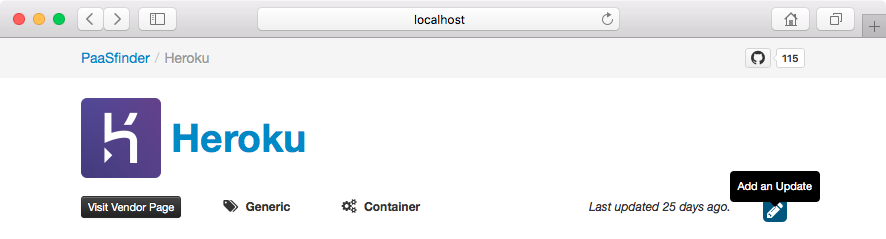
\includegraphics[width=0.95\textwidth]{images/ablauf/vendor-page.png}
		\caption{Vendor Page}
		\label{fig:vendor-page}
	\end{figure}
\item Eine neue Java Version (1.9) hinzuf�gen (siehe Abbildung \ref{fig:update-page}).
	\begin{figure}[H] 
		\centering
		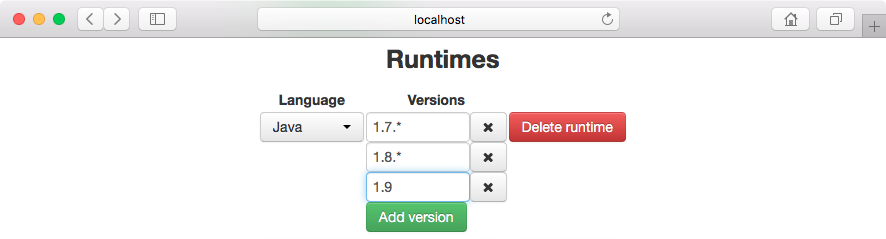
\includegraphics[width=0.95\textwidth]{images/ablauf/update-page.png}
		\caption{Update Page}
		\label{fig:update-page}
	\end{figure} 
\item Die Daten auf der Review Page �berpr�fen (siehe Abbildung \ref{fig:vendor-page}).
	\begin{figure}[H] 
		\centering
		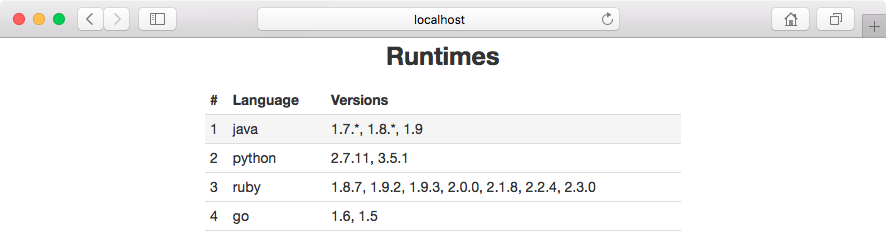
\includegraphics[width=0.95\textwidth]{images/ablauf/review-page.png}
		\caption{Review Page}
		\label{fig:review-page}
	\end{figure} 
\item Optional kann der Wissenstr�ger seine Kontaktdaten (Name und E-Mail) sowie die Nachricht zum Update hinterlassen.
	\begin{figure}[H] 
		\centering
		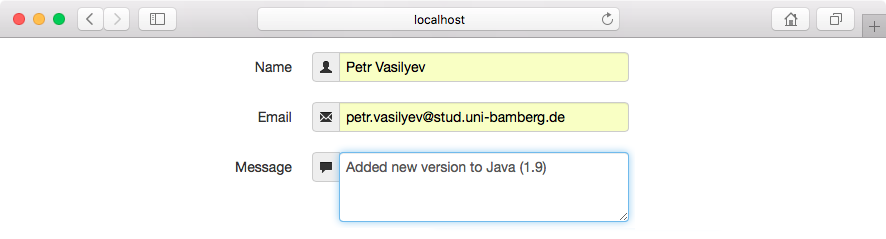
\includegraphics[width=0.95\textwidth]{images/ablauf/kontaktform.png}
		\caption{Kontaktdatenform}
		\label{fig:kontaktdatenform}
	\end{figure} 
\item Anschlie�end werden die Daten mit dem Klick auf den \glqq{}Sumbit\grqq{}-Button an die f�r die Daten�bermittlung zust�ndige Schnittstelle abgeschickt.
\end{enumerate}
Ein wichtiger Aspekt bei der Entwicklung der Wissenstr�gerschnittstelle ist die Validierung der Eingabedaten. In einigen F�llen k�nnen problematische Eingaben bereits auf der Ebene der Benutzerschnittstelle (User Interface) verhindert werden. Als Beispiel wird in der Kontaktform (Abbildung \ref{fig:kontaktdatenform}) bei der E-Mail Adresse mittels HTML-Attributes type=\glqq{}email\grqq{} sichergestellt, dass der Input formal der E-Mail Struktur einspricht. Allerdings kann der vergleichbare Ansatz nicht immer angewandt werden. Ein Beispiel ist eine Version, die ein Sonderzeichen (z.B. *) oder einen Buchstaben enthalten kann.
\subsection{Worker f�r Daten�bermittlung}\label{subsec:Worker}
Der vorliegende Abschnitt befasst sich mit einem Teil der Wissenserwerbskomponente, der als Bindeglied zwischen den Wissenserfassungsmethoden und der Wissensbasis auftritt. In Abbildung \ref{fig:wissenserwerbskomponente} wurde dieses Bindeglied allgemein als Schnittstelle f�r die Daten�bermittlung bezeichnet. Im Rahmen dieser Studie wird von einem \textit{Worker} gesprochen, der die Aufgabe der Daten�bermittlung durchf�hren wird. Der Aufgabenbereich vom Worker l�sst sich in Abbildung \ref{fig:worker} darstellen.
\begin{figure}[H] 
	\centering
	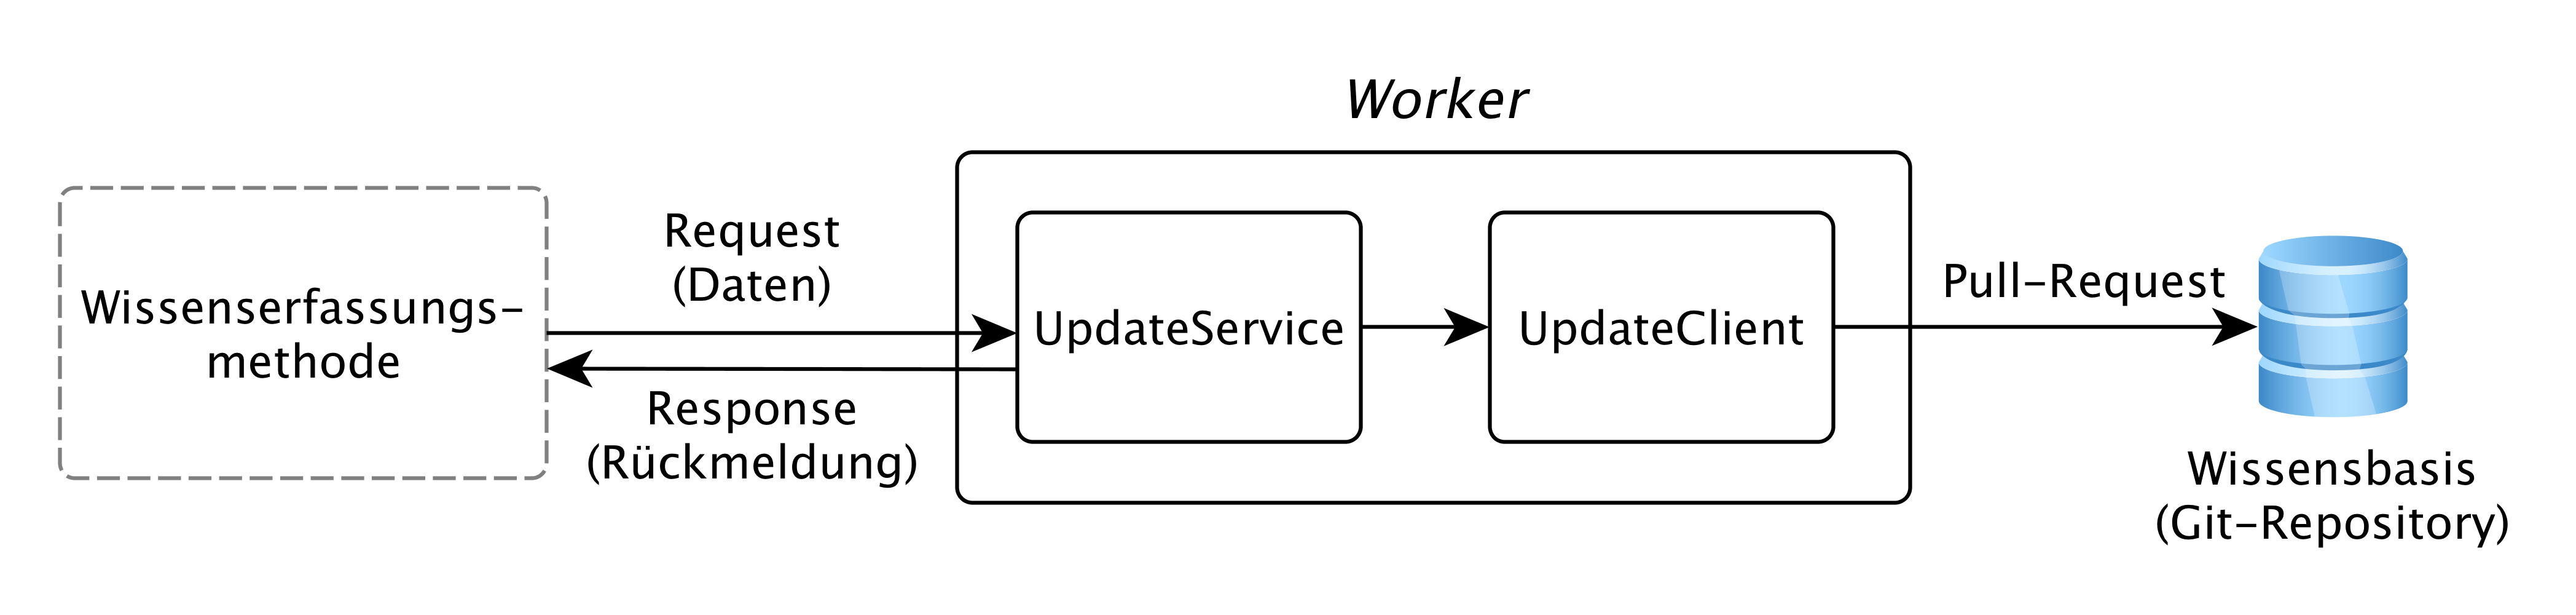
\includegraphics[width=1.0\textwidth]{images/anwendungsbereich_worker.png}
	\caption{Anwendungsbereich vom Worker}
	\label{fig:worker}
\end{figure}
In Abbildung \ref{fig:worker} sieht man, dass der Worker aus \textit{UpdateService} und \textit{UpdateClient} besteht. UpdateService stellt eine Schnittstelle dar, die f�r den Empfang der Daten zust�ndig ist. Auf der anderen Seite befasst sich UpdateClient mit der Schnittstelle der Wissensbasis (Git-Repository), um einen Pull-Request erstellen zu k�nnen.\\
Der Ablauf der Daten�bermittlung l�sst sich gem�� der Abbildung \ref{fig:worker} wie folgt beschreiben. Als erstes werden die Daten als JSON an den UpdateService geschickt (Request). Im n�chsten Schritt wird das JSON vom UpdateService verarbeitet (\glqq{}geparsed\grqq{}{}) und die Pull-Request-Erstellung an den UpdateClient delegiert. An dieser Stelle wird davon ausgegangen, dass der Pull-Request erfolgreich erstellt wurde. Der genaue Ablauf der Pull-Request-Erstellung wird im sp�teren Verlauf detaillierter angesprochen. Nachdem der Pull-Request erstellt wurde, schickt der UpdateService eine R�ckmeldung (Response) an die Wissenserfassungsmethode.\\
Die Umsetzung des Workers erfolgt auf Basis von \ac{HTTP}\footnote{https://www.w3.org/Protocols} unter Verwendung von \ac{REST}-Architekturstil, der urspr�nglich aus der Dissertation von Fielding \cite{fielding2000} stammt. Das zentrale Konzept vom Rest besteht in Ressourcen, die im globalen Raum mithilfe von \ac{URI}\footnote{https://tools.ietf.org/html/rfc3986} eindeutig identifiziert werden \cite[S.11,35]{tilkov2015}. Ein wichtiges Merkmal von REST ist die lose Kopplung zwischen dem Client und dem Server, auch als statuslose Kommunikation bezeichnet \cite[S.18]{tilkov2015}. Der Server (Worker) interessiert sich f�r den Client (Wissenserfassungsmethode) nur f�r den Zeitpunkt der Request-Verarbeitung. Danach ist der Zustand des Clients f�r den Server nicht mehr relevant.\\
Der UpdateService wird auf Basis Spark\footnote{http://sparkjava.com} umgesetzt. Spark stellt ein Micro-Framework dar, das eine kompakte, Java-basierte Implementierung von REST-API erm�glicht. Um die Daten von au�en empfangen zu k�nnen, stellt der UpdateService die \glqq{}/vendor\grqq{} Route zur Verf�gung, die vom Typ POST\footnote{https://tools.ietf.org/html/rfc7231\#section-4.3.3} ist und JSON als Medientyp erwartet.\\
Die Erstellung eines Pull-Requests erfolgt mithilfe von Github REST-API\footnote{https://developer.github.com/v3}. Diese Aufgabe wird durch den UpdateClient durchgef�hrt und setzt sich aus folgenden Schritten zusammen:
\begin{itemize}
\item[1.] \acs{SHA}-Wert vom Master-Branch holen und einen neuen Branch erstellen
\item[2.] \acs{SHA}-Wert der betroffenen JSON-Datei holen und die JSON-Datei innerhalb von Branch aktualisieren 
\item[3.] einen Pull-Request erstellen
\end{itemize}
Diese Schritte werden der UpdateClient unter Verwendung von OkHttp\footnote{https://square.github.io/okhttp} implementiert und dem UpdateService als Methoden zur Verf�gung gestellt.\\
%Im folgenden Beispiel wird der Ablauf der Aktualisierung von dargestellt 
\textit{Beispiel beschreiben}
\newpage
\subsection{Webcrawler}
Ausf�hren
\section{Evaluation}\label{sec:Evaluation}
\subsection{Test 1}
\subsection{Test 2}
\subsection{Test 3}
\section{Ausblick}\label{sec:Ausblick}
\newpage

% Einstellungen f�r Literaturverzeichnis
\addcontentsline{toc}{section}{\bibname}
\bibliographystyle{geralpha}
\selectlanguage{german}

% Hier das Literaturverzeichnis einbinden
\bibliography{bibliography/references}
\newpage

% Eigenst�ndigkeitserkl�rung
\makedeclaration{Bachelorarbeit}{31.03.2017}{Petr Vasilyev}

\end{document}